% SVN info for this file
\svnidlong
{$HeadURL$}
{$LastChangedDate$}
{$LastChangedRevision$}
{$LastChangedBy$}

\chapter{Coniche proiettive}
\labelChapter{conicheproiettive}

\begin{introduction}
	‘‘BEEP BOOP INSERIRE CITAZIONE QUA BEEP BOOP.''
	\begin{flushright}
		\textsc{NON UN ROBOT,} UN UMANO IN CARNE ED OSSA BEEP BOOP.
	\end{flushright}
\end{introduction}
%inserire citazione
Nella geometria Euclidea le \textbf{coniche} sono curve ottenute dall'intersezione di un \textit{cono} con un \textit{piano}. Nel piano affine $\mathcal{A}(\realset^2)$ si generalizzano (includendo anche casi degeneri) studiando le \textit{forme quadratiche} e classificandole \textit{a meno di rototraslazione}. Vogliamo estendere ulteriormente il al \textit{piano proiettivo} di queste coniche, tenendo dunque conto del ruolo svolto dalla \textit{retta all'infinito}.
\section{Curve algebriche piane proiettive}
Consideriamo $\proj[2]{\kamp}$ con coordinate omogenee $(x_0\colon x_1\colon x_2)$. Indichiamo con $\kamp\left[x_0,\ x_1,\ x_2\right]$ l'\textit{anello dei polinomi} in $x_0,\ x_1,\ x_2$ a coefficienti in $\kamp$. Se $F\in\kamp\left[x_0,\ x_1,\ x_2\right]$ è un polinomio \textit{qualsiasi}, l'equazione $F(x_0,\ x_1,\ x_2)=0$ \textit{non} dà una condizione \textit{ben definita} in $\proj[2]{\kamp}$: ad esempio, $x_0+1=0$ non ha senso perché $x_0$ è determinato solo a meno di multipli. Cerchiamo dunque dei polinomi che ha senso studiare in $\proj[2]{\kamp}$.
\begin{define}[Polinomio omogeneo.]~{}\\
Sia $F\in\kamp\left[x_0,\ x_1,\ x_2\right]$ un polinomio. Si dice che $F$ è un \textbf{polinomio omogeneo}\index{polinomio!omogeneo} se tutti i monomi a coefficienti \textit{non} nulli hanno lo \textit{stesso} grado.
\end{define}
% Notiamo che la definizione è significativa per polinomi a più variabili, altrimenti i polinomi omogenei sarebbero solo monomi. (non ho questa nota :/)
\begin{examples}~{}
	\begin{itemize}
		\item $F=x_0^3+x_0x_1^2-3x_1x_2x_3\in\realset\left[x_0,\ x_1,\ x_2\right]$ è un polinomio omogeneo di grado $3$.
		\item $G=x_0^3-x_1x_2+1$ non è un polinomio omogeneo.
	\end{itemize}
\vspace{-3mm}
\end{examples}

\begin{observe}
Se $\deg F=1$, cioè $F=a_0x_0+\ldots+a_nx_n+b$, allora $F$ è omogeneo se e solo se $b=0$.
\end{observe}

\begin{observe}
Se $F\in\kamp\left[x_0,\ x_1,\ x_2\right]$ è omogeneo di grado $d$ allora:
\begin{equation}
F(\lambda x_0,\ \lambda x_1,\ \ldots,\ \lambda x_n)=\lambda^d F(x_0,\ \ldots,\ x_n)
\end{equation}
Infatti, $F$ è somma di monomi di grado $d$ del tipo $ax_0^{i_0}x_1^{i_1}\cdots x_n^{i_n}$ con $\displaystyle\sum_{j=0}^n i_j=d$ e si ha che $a(\lambda x_0)^{i_0} (\lambda x_1)^{i_1} \cdots (\lambda x_n)^{i_n}=\lambda^{i_0+\ldots +i_n} (ax_0^{i_0}\ldots x_n^{i_n})=\lambda^d(ax_0^{i_0}\ldots x_n^{i_n})$.
\end{observe}
Torniamo al piano proiettivo $\proj[2]{\ }$ con le coordinate omogenee $(x_0\colon x_1\colon x_2)$ e consideriamo $F\in\kamp\left[x_0,\ x_1,\ x_2\right]$ un polinomio omogeneo nelle coordinate omogenee di grado $d$. Se abbiamo un punto $P=(c_0\colon c_1\colon c_2)\in\proj[2]{\ }$, allora tutte le possibili scelte per le coordinate di $P$ sono $(\lambda c_0\colon \lambda c_1 \colon \lambda c_2)$ con $\lambda\in\kamp\setminus\{0\}$. Valutando $F$ in $P$, otteniamo $F(\lambda c_0,\ \lambda c_1,\ \lambda c_2)=\lambda^d F(c_0,\ c_1,\ c_2)$: in altre parole, $F$ si annulla in una scelta di coordinate se e solo se si annulla in qualsiasi scelta di coordinate, cioè:
\begin{equation*}
F(c_0,\ c_1,\ c_2)=0\iff F(\lambda c_0,\ \lambda c_1,\ \lambda c_2)=0,\ \forall \lambda\in\kamp\setminus\{0\}
\end{equation*}
Pertanto, l'equazione $F(x_0,\ x_1,\ x_2)=0$ è ben posta in $\proj[2]{\ }$.
\begin{example}
$x_0^2-x_1x_2=0$ definisce un sottoinsieme del piano proiettivo.
\end{example}
\begin{define}[Curva algebrica piana proiettiva.]~{}\\
	Una \textbf{curva algebrica piana proiettiva}\index{curva!algebrica!proiettiva} $C$ di $\proj[2]{\ }$ è il luoghi degli zeri dato da un polinomio omogeneo $F\in\kamp\left[x_0,\ x_1,\ x_2\right]$:
	\begin{equation}
		C=\left\{(x_0,\ x_1,\ x_2)\in\proj[2]{\ }\mid F(x_0,\ x_1,\ x_2)=0\right\}
	\end{equation}
	La curva è definita a meno di multipli: se $G=\lambda F$ con $\lambda\in\kamp\setminus\left\{0\right\}$, $G$ e $F$ descrivono la stessa curva.\\
	Diciamo che la curva $C$ è \textbf{reale} se $\kamp=\realset$ (e quindi $C\in\proj[2]{\realset}$), \textbf{complessa} se $\kamp=\complexset$ (e quindi $C\in\proj[2]{\complexset}$).
\end{define}
\begin{define}[Equazione di una curva.]~{}\\
	L'\textbf{equazione}\index{equazione!di una curva} di una curva $C$ è il polinomio $F$ (a a meno di multipli) che la descrive.
\end{define}
\begin{define}[Supporto di una curva.]~{}\\
	Il \textbf{supporto}\index{supporto} di una curva $C$ descritta da un polinomio $F$ (a a meno di multipli) è l'insieme dove il polinomio si annulla.\\
	L'equazione determina il supporto, ma in generale non vale il contrario.
\end{define}
\begin{define}[Grado di una curva.]~{}\\
	Il \textbf{grado}\index{grado!di una curva} della curva $C$ è il grado dell'equazione $F$.
\end{define}
\begin{example}
	Preso il polinomio $F(x_0,\ x_1,\ x_2)=a_0x_0+a_1x_1+a_2x_2=0$,la curva $C$ descrive una retta.
\end{example}
\begin{define}[Rette e coniche proiettive.]~{}
	\begin{itemize}
		\item Le \textbf{rette proiettive} sono curve di grado $1$.
		\item Le \textbf{coniche proiettiva} sono curve di grado $2$.
	\end{itemize}
\vspace{-3mm}
\end{define}
%LEZ 33
D'ora in poi ci restringeremo ai casi $\kamp=\realset$ e $\kamp=\complexset$.
\begin{define}[Curva irriducibile.]~{}\\
Una curva $C$ è \textbf{irriducibile}\index{curva!irriducibile} se lo è la sua equazione $F$. Altrimenti si considera la sua fattorizzazione in irriducibili:
\begin{equation}
	F=F_1^{m_1}\cdot \ldots \cdot F_r^{m_r}
\end{equation}
Siccome ogni fattore irriducibile $F_i$ è omogeneo, ognuno definisce una curva $C_i\colon F_i=0$, dette \textbf{componenti irriducibili}\index{componenti irriducibili della curva} della curva $C$.\\
Se $m_i>1$ diciamo che $C_i$ è una componente di \textbf{molteplicità}\index{molteplicità} $m_i$ in $C$
\end{define}

\begin{examples}
	\begin{itemize}
		\item Le rette, essendo curve di grado 1, sono \textit{sempre} \textbf{irriducibili}.\\
		Le coniche sono curve di grado 2. Dunque, considerata una conica $C$ di equazione $F=0$, ci sono 3 possibilità:
		\begin{enumerate}
			\item	$C$ è \textbf{irriducibile}.
			\item	$C$ è il prodotto di fattori lineari distinti e non multipli:
			\begin{equation}
				F=L_1\cdot L_2
			\end{equation}
			Con $L_i$ forme lineari \textit{non} proporzionali. Pertanto, $C$ è una \textbf{coppia di rette distinte} (ad es. $C\colon F=x_0x_1\implies C$ unione delle rette $x_0=0$ e $x_1=0$).
			\item	$C$ è data da fattori lineari associati, cioè $F$ è un quadrato a meno di uno scalare:
			\begin{equation}
				F=\lambda L^2,\ \lambda\in\kamp\setminus\{0\}
			\end{equation}
			Allora $C$ è una \textbf{retta doppia}: la retta è la sola componente irriducibile ed è di molteplicità 2 (ad es. $C\colon F=x_0^2$).
		\end{enumerate}
	\end{itemize}
\vspace{-3mm}
\end{examples}

\section{Coniche proiettive}
\begin{define}[Conica.]~{}\\
		Una \textbf{conica}\index{conica} $C$ di $\proj[2]{\ }$ è il luoghi degli zeri dato da un polinomio omogeneo $F\in\kamp\left[x_0,\ x_1,\ x_2\right]$ di grado 2 in $x_0,\ x_1,\ x_2$ a coefficienti \textit{reali} o \textit{complessi}.
		\begin{equation*}
			F=a_{00}x_0^2 +a_{01}x_0x_1+a_{02}x_0x_2+a_{11}x_1^2+a_{12}x_1x_2+a_{22}x_2^2
		\end{equation*}
\end{define}
In generale, i polinomi omogenei di grado 2 sono \textit{forme quadratiche}. Pertanto, vogliamo associare alla forma la  corrispondente matrice simmetrica.
%forma <---> polinomio omogeneo
Per evitare di dividere per 2 i termini misti, ci è lecito immaginarli già nella forma $2a_{01},\ 2a_{02},\ 2a_{12}$, ottenendo così:
\begin{equation*}
F=a_{00}x_0^2 +2a_{01}x_0x_1+2a_{02}x_0x_2+a_{11}x_1^2+2a_{12}x_1x_2+a_{22}x_2^2
\end{equation*}
Allora la matrice simmetrica $3\times 3$ associata alla forma quadratica è:
\begin{equation}
	A=(a_{ij})=\left(\begin{array}{ccc}
		a_{00} & a_{01} & a_{02}\\
		a_{01} & a_{11} & a_{12}\\
		a_{02} & a_{11} & a_{22}\\
	\end{array}\right)\in S\left(\kamp^{3,3}\right)
\end{equation}
Ed è tale per cui $\displaystyle F=x^tAx$ con $x=\left( \begin{array}{c}
x_0 \\ x_1 \\ x_2
\end{array} \right)$ il vettore delle coordinate omogenee.\\
\begin{define}[Rango della conica.]~{}\\
Il \textbf{rango}\index{rango!di una conica} della conica $C$ è il rango della matrice associata $A$.
\end{define}
\begin{observe}
Come già osservato, l'equazione della conica $C$ determina $F$ solo a meno di multipli, dunque anche la matrice $A$ è determinata \textit{a meno di multipli}.
Tuttavia, il rango rimane ben definito in quanto $\rk(\lambda A)=\rk(A),\ \forall\lambda\neq 0$. Inoltre, il rango \textit{non} può essere $0$ perché essendo l'equazione di una conica il polinomio \textit{non} può essere nullo (non descriveremmo una conica!).
\end{observe}
Vogliamo studiare le coniche e le curve di grado maggiore a meno di equivalenza proiettiva, allo stesso modo in cui abbiamo classificato le coniche in $\realset^2$ a meno di rototraslazioni.\\
Sia dunque $\funz f {\proj[2]{\ }} {\proj[2]{\ }}$ una proiettività, la cui matrice associata $M\in\gl(3,\kamp)$ è tale per cui $x'=Mx$. Allora $f$ porta la conica $C\colon F=0$ nella conica $\widetilde{C}\colon \widetilde{F}=0$, dove $\widetilde{F}$ si ottiene sostituendo in $f$ il vettore $x=M^{-1}x'$.
\begin{example}
Sia $C \colon x_ox_1=0$ una coppia di rette e $f$ una proiettività tale che:
\begin{equation*}
	f(x_0\colon x_1\colon x_2)=(x_0+x_1\colon x_0-2x_1\colon x_2)
\end{equation*}
Scriviamo, usando la matrice associata alla proiettività, il vettore immagine $x'_i$ in funzione di $x_i$ e poi ricaviamo $x_i$ in funzione di $x'_i$.
\begin{gather*}
f\colon \begin{cases}
x'_0=x_0+x_1\\
x'_1=x_0-2x_2\\
x'_2=x_2
\end{cases} \implies \begin{cases}
-3x_1=x'_1-x'_0 \implies x_1=\frac{1}{3}(x'_0-x'_1)\\
x_0=x'_0-x_1=x'_0 -\frac{1}{3}(x'_0-x'_1)=\frac{1}{3}(2x'_0+x'_1)
\end{cases}\\
f^{-1}\colon \begin{cases}
x_0=\frac{1}{3}(2x'_0+x'_1)\\
x_1=\frac{1}{3}(x'_0-x'_1)\\
x_2=x'_2
\end{cases}
\end{gather*}
In sostanza abbiamo ottenuto l'espressione dell'inversa di $f$; quindi, la trasformata di $C$ tramite $f$ è $(2x_01+)(x'_0-x'_1)=0$, che è ancora una coppia di rette. In particolare, notiamo che esse sono le immagini tramite $f$ delle rette $x_0=$ e $x_1=0$, a meno dei fattori moltiplicativi $\frac{1}{3}$.
\end{example}
Osserviamo che la proiettività manda il supporto della prima conica nel supporto della seconda conica e che, trasformando la conica tramite una proiettività, trasformiamo la forma quadratica $F$ tramite un cambiamento di coordinate di $\kamp^3$.\\
Dunque, se $A$ è la matrice associata a $C$ e $\widetilde{A}$ è la matrice associata alla trasformata $\widetilde{C}$ tramite $f$, allora $A$ e $\widetilde{A}$ sono \textbf{congruenti}.
Infatti, il \textit{cambiamento di coordinate} su uno spazio vettoriale per la forma quadratica è dato da $\widetilde{A}=M^tAM$ con $M\in\gl\left(3,\kamp\right)$ con $M$ una matrice associata della proiettività, interpretata come matrice del cambiamento di base.\\
Viceversa, date due coniche $C_1$ e $C_2$ le cui matrici associate (simmetriche) $A_1$ e $A_2$ sono congruenti, allora $C_1$ e $C_2$ sono \textit{proiettivamente equivalenti}:  questo perché, in generale, forme quadratiche congruenti differiscono per un cambiamento di base.\\ Otteniamo così la seguente corrispondenza:
\begin{equation*}
\begin{array}{ccc}
C_1\text{ e }C_2\text{ equivalenti}& \iff & A_1\text{ e }A_2\text{ congruenti}
\end{array}
\end{equation*}
Pertanto lo studio delle coniche, a meno di equivalenze proiettive, passa per lo studio delle matrici congruenti.
\subsection{Classificazione delle coniche proiettive complesse}
\begin{remember}
Nel campo dei complessi ($\kamp=\complexset$) due matrici simmetriche \textit{sono congruenti} se e solo se hanno lo \textit{stesso rango}.
\begin{equation*}
	\begin{array}{ccc}
		A_1\text{ e }A_2\text{ congruenti}& \iff & \rk A_1=\rk A_2
	\end{array}
\end{equation*}
In generale, vale solo che se le matrici simmetriche sono congruenti allora hanno lo stesso rango (ma non il viceversa!).
\end{remember}
Allora, a meno di equivalenza proiettiva, ci sono solo 3 possibili coniche: quelle di rango 1, rango 2 e rango 3.
\begin{theorema}[Classificazione delle coniche proiettive complesse.]~{}\\
\begin{enumerate}
\item	Due coniche in $\proj[2]{\complexset}$ sono proiettivamente equivalenti se e solo se hanno lo stesso rango.
\item	\textbf{Forma canonica}: ogni conica di $\proj[2]{\complexset}$ è proiettivamente equivalente ad \textit{una ed una sola} delle tre coniche seguenti:\\
\begin{equation*}
		\begin{array}{cll}
		\underline{\rk 3}\colon & x_0^2+x_1^2+x_3^2=0 &	\text{Conica irriducibile}\\[1mm]
		\underline{\rk 2} \colon & x_0^2+x_1^2=(x_0+ix_i)(x_0-ix_1)=0 & \text{Coppia di rette distinte}\\[1mm]
		\underline{\rk 1} \colon & x_0^2=0 & \text{Retta doppia}
	\end{array}
\end{equation*}
\end{enumerate}
\vspace{-3mm}
\end{theorema}

%questo è dato dalla classificazione delle forme quadratiche du \complexset^3

v\subsection{Classificazione delle coniche proiettive reali}
Sia $C$ una conica in $\proj[2]{\realset}$ con matrice associata $A$, simmetrica \textit{reale} $3\times 3$. Come abbiamo detto, poiché la matrice non è complessa, non è sufficiente il rango per la congruenza: affinché sia congruente ad un'altra matrice simmetrica serve anche la \textbf{segnatura}.
\begin{observe}
Siccome $A$ è determinata a meno di multipli, in principio la segnatura potrebbe cambiare. Vediamo cosa succede effettivamente.\\
Se $A$ ha segnatura $(p,q)$ con $p$ il numero di autovalori \textit{positivi} e $q$ il numero di autovalori \textit{negativi}, allora $\lambda A$ può avere segnatura $(p,q)$ se $\lambda>0$ oppure $(q,p)$ se $\lambda <0$.\\
Quindi, la segnatura di una conica è definita solo ‘‘a meno del segno'', nel senso che $(p,q)=(q,p)$.
\end{observe}
\begin{theorema}[Classificazione delle coniche proiettive reali.]~{}
	\begin{enumerate}
	\item	 Due coniche in $\proj[2]{\realset}$ sono proiettivamente equivalenti se e solo se hanno la stessa \textit{segnatura} a meno del segno; dalla segnatura si deduce anche il \textit{rango}.
	\item	Ogni conica in $\proj[2]{\realset}$ è proiettivamente equivalente a una ed una sola delle seguenti coniche, con segnature distinte a meno del segno:
	\begin{equation*}
		\arraycolsep=2.5pt
		\begin{array}{ccll}
			\underline{\rk 3} & \begin{array}{l}
					(3,0)/(0,3) \\
					\\
					(1,2)/(2,1)
				\end{array} & \begin{array}{l}
				x_0^2+x_1^2+x_2^2=0\\
				\\
				x_0^2+x_1^2-x_2^2=0\\
			\end{array}
				 & \begin{array}{l}
			\begin{array}{l}
				\text{Conica irriducibile senza} \\
				\text{punti reali (supporto vuoto)}
			\end{array} \\
			\begin{array}{l}
				\text{Conica irriducibile a punti reali,} \\
				\text{contiene infiniti punti in }\proj[2]{\realset}
			\end{array}
		\end{array}\\ \hline %ha un supporto? ci sono dei punti in P2R che hanno questa equazione? no perché escludiamo l'origine	conica irriducibile senza punti reali /tipo ellisse immaginario/ dunque il supporto è vuoto
		\underline{\rk 2} &\begin{array}{c}
		(2,0)/(0,2) \\
		\\
		(1,1)
		\end{array} &\begin{array}{l}
		\\[-1mm]
		x_0^2+x_1^2=0 \\
		\\[-1mm]
		x_0^2-x_1^2=\\[-0.75ex]
		=(x_0-x_1)(x_0+x_1)=0
		\end{array} & \begin{array}{l}
		\begin{array}{l}
		\text{Coppia di rette non reali} \\
		\text{con } 1 \text{ punto reale } (0\colon 0\colon 1)
		\end{array} \\ %	perché si fattorizza ma a coeff complessi. Ha un unico punto reale (0\colon 0\colon 1) intersezione delle due rette complesse coniugate
		\begin{array}{l}
		\text{Conica irriducibile a punti reali,} \\
		\text{coppia di rette reali distinte}
		\end{array}
		\end{array} \\[2mm] \hline %che si fattorizza su R
		\underline{\rk 1} & (1,0) & \begin{array}{l}
			\\[-4mm]
			x_0^2=0
		\end{array} &\ \ \begin{array}{l}
		\text{Retta doppia}
	\end{array}	
\end{array}	
	\end{equation*}
	\end{enumerate}
\end{theorema}

\section{Curve algebriche piane affini e chiusura proiettiva}
Siccome abbiamo interpretato il piano proiettivo come un'\textit{estensione} di quello affine, possiamo confrontare la classificazione delle curve nel piano proiettivo con la \textit{classificazione nel caso affine}.
\begin{define}[Curva algebrica piana affine.]~{}\\
	Una \textbf{curva algebrica piana affine}\index{curva!algebrica!affine} $C$ di $\aff{\kamp^2}$ è il luoghi degli zeri dato da un polinomio omogeneo $f\in\kamp\left[x,\ y\right]$:
\begin{equation}
	C=\left\{\left(x,\ y\right)\in\proj[2]{\ }\mid f\left(x,\ y\right)=0\right\}
\end{equation}
La curva è definita a meno di multipli: se $g=\lambda f$ con $\lambda\in\kamp\setminus\left\{0\right\}$, $g$ e $f$ descrivono la stessa curva.\\
Diciamo che la curva $C$ è \textbf{reale} se $\kamp=\realset$ (e quindi $C\in\aff{\realset^2}$), \textbf{complessa} se $\kamp=\complexset$ (e quindi $C\in\aff{\complexset^2}$).
\end{define}
\begin{define}[Equazione di una curva.]~{}\\
L'\textbf{equazione}\index{equazione!di una curva} di una curva $C$ è il polinomio $f$ (a a meno di multipli) che la descrive.
\end{define}
\begin{define}[Supporto di una curva.]~{}\\
Il \textbf{supporto}\index{supporto} di una curva $C$ descritta da un polinomio $f$ (a a meno di multipli) è l'insieme dove il polinomio si annulla.\\
L'equazione determina il supporto, ma in generale non vale il contrario.
\end{define}
\begin{define}[Grado di una curva.]~{}\\
Il \textbf{grado}\index{grado!di una curva} della curva $C$ è il grado dell'equazione $f$.
\end{define}
\begin{define}[Curva irriducibile.]~{}\\
	Una curva $C$ è \textbf{irriducibile}\index{curva!irriducibile} se lo è la sua equazione $f$. Altrimenti si considera la sua fattorizzazione in irriducibili:
	\begin{equation}
		f=f_1^{m_1}\cdot \ldots \cdot f_r^{m_r}
	\end{equation}
	Siccome ogni fattore irriducibile $f_i$ è omogeneo, ognuno definisce una curva $C_i\colon f_i=0$, dette \textbf{componenti irriducibili}\index{componenti irriducibili della curva} della curva $C$.\\
	Se $m_i>1$ diciamo che $C_i$ è una componente di \textbf{molteplicità}\index{molteplicità} $m_i$ in $C$
\end{define}
\begin{define}[Rette e coniche affini.]~{}
	\begin{itemize}
		\item Le \textbf{rette affini} $ax+by+c=0$ sono curve di grado $1$.
		\item Le \textbf{coniche affini} $ax^2+by^2+cxy+dx+ey+f=0$ sono curve di grado $2$.
	\end{itemize}
	\vspace{-3mm}
\end{define}
\subsubsection{Omogeneizzazione di un polinomio}
Vediamo ora qual è il legame fra curve affini e proiettive utilizzando la \textit{chiusura proiettiva}. Ricordiamo che $\kamp^2=U_0\subset \proj[2]{\kamp}$ con $\left(x,\ y\right)\in\kamp^2$ che corrispondono a $\displaystyle x=\frac{x_1}{x_0}$ e $\displaystyle y=\frac{x_2}{x_0}$, dato $(x_0\colon x_1\colon x_2)\in\proj[2]{\kamp}$.\\
Sia $C$ una curva affine di equazione $f\left(x,\ y\right)=0$. Vogliamo associare a $f$ un polinomio omogeneo nelle coordinate $x_0,\ x_1,\ x_2$ dello stesso grado di $f$.
Consideriamo dunque il polinomio $F\in\kamp\left[x_0,\ x_1,\ x_2\right]$ così definito: se $d=\deg f$, allora:
\begin{equation}
	F\coloneqq x_0^d f\left( \frac{x_1}{x_0}, \frac{x_2}{x_0} \right)
\end{equation}
Esso è a tutti gli effetti un polinomio dello stesso grado di $f$. Infatti, $F$ è un polinomio omogeneo di grado $d$: considerato un monomio in $f$, della forma $ax^iy^j$, allora $i+j$ se ne ottiene uno di grado $d$ in $x_0,\ x_1,\ x_2$:
	\begin{equation*}
		ax^iy^j \Longrightarrow x_0^d a \left( \frac{x_1}{x_0} \right)^i \left( \frac{x_2}{x_0} \right)^j = ax_0^{d-i-j} x_1^i x_2^j
	\end{equation*}
Ripetendo questa procedura per ogni monomio si ottiene un polinomio omogeneo $f$ di grado $d$ come desiderato. Notiamo che, operativamente, l'omogeneizzazione consiste nel cambiare nome alle variabili $x$ e $y$ e moltiplicare per un'opportuna potenza di $x_0$ in modo tale che il monomio sia di grado $d$.
\begin{example} Vogliamo omogenizzare il polinomio $f=x^3-2xy+3y+1$. Prima di tutto si cambia il nome delle variabili e si ottiene $x_1^3-2x_1x_2+3x_2+1$. Moltiplicando ciascun monomio per l'opportuna potenza di $x_0$, il polinomio omogeneizzato rispetto a $x_0$ sarà $F=x_1^3-2x_0x_1x_2 +3x_0^2x_2+x_0^3$.
\end{example}
\begin{observe}
	Possiamo ‘‘deomogeneizzare'' un polinomio omogeneo $F(x_0,\ x_1,\ x_2)$: ponendo $x_0=1$ si riottiene il polinomio di partenza $f(x_1,\ x_2)$.
\end{observe}
\subsubsection{Chiusura proiettiva}
\begin{define}[Chiusura proiettiva di una curva affine.]~{}\\
	La curva $\overline{C}$ in $\proj[2]{\kamp}$ definita da $F=0$ si dice \textbf{chiusura proiettiva}\index{chiusura!proiettiva!di una curva} della curva affine $C$ di equazione $f=0$.
\end{define}
Se $P=(1\colon x\colon y)\in U_0$  allora $f\left(x,\ y\right)=F\left(P\right)$ e in particolare $\overline{C}\cap U_0=C$.
\begin{define}[Punti impropri di una curva.]~{}\\
	I \textit{punti impropri} o \textit{punti all'infinito} della curva $C$ sono dati dall'intersezione della chiusura proiettiva con la \textit{retta impropria}, ovvero da $\overline{C}\cap\{x_0=0\}$
\end{define}
\begin{example}\textsc{Chiusura proiettiva di una retta}.\\
	Se $C$ è una retta $ax+by+c=0$, allora la \textit{chiusura proiettiva} di $C$ è $ax_1+bx_2+cx_0=0$ ed il \textit{punto improprio} di $C$ è $(0\colon -b\colon a)$, che corrisponde alla direzione della retta $C$.
\end{example}

\begin{examples}
	Consideriamo in $\realset^2$ le coniche:
	\begin{equation*}
		\begin{array}{cll}
			C_1\colon & y=x^2 & 	\text{Parabola}\\[1mm]
			C_2\colon & x^2+y^2=1 &		\text{Circonferenza}\\[1mm]
			C_3\colon &	x^2-y^2=1 & \text{Iperbole}
		\end{array}
	\end{equation*}
	Consideriamo ora le loro \textit{chiusure proiettive reali} tramite l'omogeneizzazione, cioè le coniche proiettive $\overline{C_i}$ in $\proj[2]{\realset}$:
		\begin{equation*}
		\begin{array}{cl}
			\overline{C_1} \colon & x_0x_1=x_1^2\\[1mm]
			\overline{C_2} \colon & x_1^2+x_2^2=x_0^2\\[1mm]
			\overline{C_3} \colon & x_1^2-x_2^2=x_0^2
		\end{array}
	\end{equation*}
	Scrivendo le matrici associate e guardandone la segnatura, si vede che \textit{tutte e tre} hanno segnatura $(2,1)/(1,2)$ e quindi tutte proiettivamente equivalenti (per la classificazione delle coniche nel piano proiettivo reale) ad una \textit{conica irriducibile a punti reali} in $\proj[2]{\realset}$.\\
	Consideriamo ora i loro punti impropri:
		\begin{itemize}
			\item \textsc{Parabola}: $\overline{C_1}\cap\{x_0=0\}\colon (0\colon 0\colon 1)$, dunque un solo punto improprio, ovvero la direzione $(0,1)$ dell'asse $y=\mathcal{L}(0,1)$, quindi è l'asse della parabola
			\item \textsc{Circonferenza}: $\overline{C_2}\cap \{x_0=0\} \colon x_0=0 \implies x_1=x_2=0$ ma non si possono avere tute le coordinate omogenee nulle, dunque non ci sono punti impropri
			\item \textsc{Iperbole}: $\overline{C_3}\cap\{x_0=0\}\colon x_1^2-x_2^2=0$, dunque ci sono	due punti impropri quali $(0\colon 1\colon 1)$ e $(0\colon 1\colon -1)$, a cui corrispondono le direzioni degli asintoti dell'iperbole
		\end{itemize}
	Notiamo che le chiusure proiettive viste sono tutte proiettivamente equivalenti, ma hanno 3 posizioni diverse rispetto alla \textit{retta impropria}:\\
			\begin{minipage}{0.57\textwidth}
			\begin{enumerate}[series=proj2]
				\item $\overline{C_1}$ è ‘‘\textit{tangente}'' alla retta impropria.
			\end{enumerate}
		\end{minipage}
		\begin{minipage}{0.52\textwidth}
					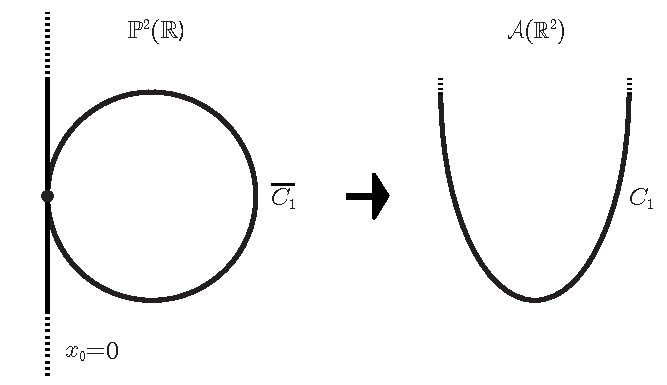
\includegraphics[trim=0cm 0cm 0cm 0cm,clip,scale=0.50]{images/projconic1.pdf}
		\end{minipage}\\
	\begin{minipage}{0.57\textwidth}
		\begin{enumerate}[resume=proj2]
		\item $\overline{C_2}$ è ‘‘\textit{disgiunta}'' dalla retta impropria.
		\end{enumerate}
	\end{minipage}
	\begin{minipage}{0.52\textwidth}
					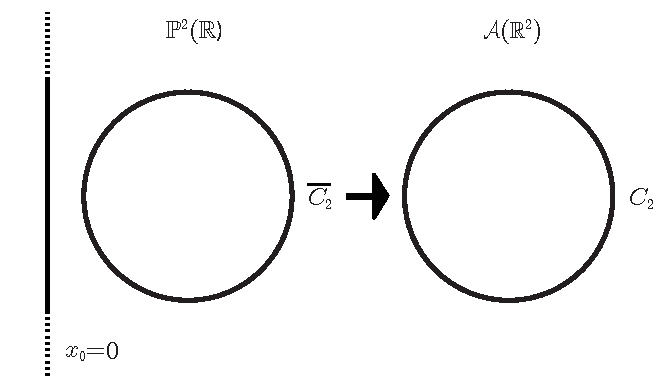
\includegraphics[trim=0cm 0cm 0cm 0cm,clip,scale=0.50]{images/projconic2.pdf}
	\end{minipage}\\
	\begin{minipage}{0.57\textwidth}
	\begin{enumerate}[resume=proj2]
		\item $\overline{C_3}$ è ‘‘\textit{secante}'' rispetto alla retta impropria.
	\end{enumerate}
\end{minipage}
\begin{minipage}{0.52\textwidth}
					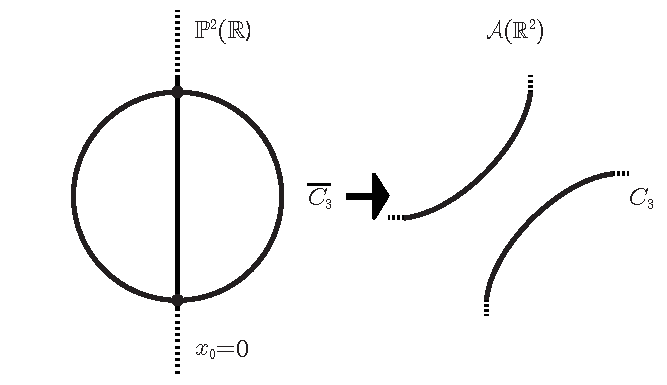
\includegraphics[trim=0cm 0cm 0cm 0cm,clip,scale=0.50]{images/projconic3.pdf}
\end{minipage}
\end{examples}
\begin{example}
	In $\aff{\realset^2}$ consideriamo la coppia di \textit{rette parallele} distinte $x(x+1)=0$ e la coppia di \textit{rette incidenti} distinte $xy=0$.\\
	Prendendo le le chiusure proiettive si ottiene $x_1(x_1+x_0)=0$ e $x_1x_2=0$, entrambe coppie di rette distinte reali in $\proj[2]{\realset}$ con segnatura (1,1). \\
	Dunque sono proiettivamente equivalenti fra loro ma hanno posizione diversa rispetto alla retta impropria.
	\begin{itemize}
		\item La prima ha un solo punto improprio $(0\colon 0\colon 1)$, che è la \textit{direzione comune} delle due rette parallele nel piano affine.
		\begin{center}
			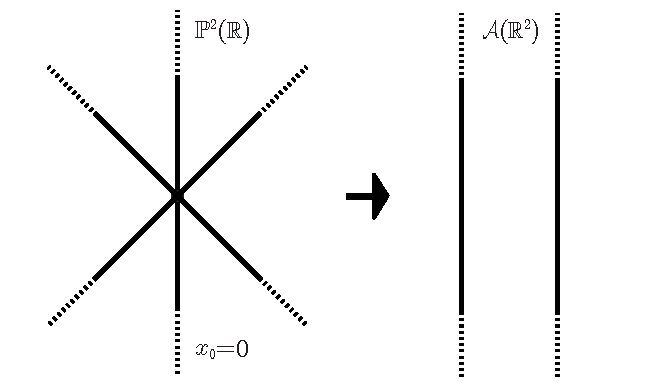
\includegraphics[trim=0cm 0cm 0cm 0cm,clip,scale=0.50]{images/projlineintersect1.pdf}
		\end{center}
		\item La seconda ha due punti impropri $(0\colon 0\colon 1)$ e $(0\colon 1\colon 0)$, che sono le direzioni delle due rette nel piano affine.
		\begin{center}
			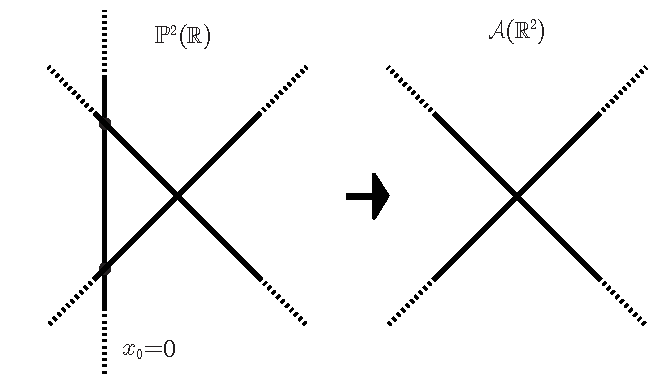
\includegraphics[trim=0cm 0cm 0cm 0cm,clip,scale=0.50]{images/projlineintersect2.pdf}
		\end{center}
	\end{itemize}
\vspace{-3mm}
\end{example}
\section{Classificazione affine delle coniche nel caso complesso}
Ragionando dalla classificazione delle coniche proiettive si può mettere in relazione la classificazioni delle coniche affini $\aff{\complexset^2}$ (a meno di rototraslazione), prestando attenzione alla posizione rispetto alla retta impropria.
\begin{proposition}[Classificazione delle coniche affini complesse.]~{}\\
Ogni conica in $\complexset^2$ si può ridurre con una trasformazione del tipo:
\begin{equation}
	\begin{pmatrix} x' \\ y' \end{pmatrix} =A\begin{pmatrix} x \\ y \end{pmatrix} +b
\end{equation}
Con $b\in\complexset^2$ e $A\in\gl(2,\complexset)$ ad una delle cinque coniche:
\begin{center}
	\begin{tabular}{cll}
	1. &	$x^2+y^2+1=0$ & \begin{tabular}{l}
			${\scriptstyle \blacksquare}$ Rango 3.\\
			${\scriptstyle \blacksquare}$ \textit{Due} punti impropri \textit{distinti}.
		\end{tabular}   \\ \hline
	2. &	$y-x^2=0$ & \begin{tabular}{l}
			${\scriptstyle \blacksquare}$ Rango 3.\\
			${\scriptstyle \blacksquare}$ Un \textit{unico} punto improprio.
		\end{tabular}  \\ \hline
	3. &	$x^2+y^2=(x+iy)(x-iy)=0$ & \begin{tabular}{l}
			Coppia di rette distinte \textit{incidenti}:\\
			${\scriptstyle \blacksquare}$ Rango 2.\\
			${\scriptstyle \blacksquare}$ \textit{Due} punti impropri \textit{distinti}.
		\end{tabular} \\ \hline
	4. &	$x(x+1)=0$ & \begin{tabular}{l}
			Coppia di rette distinte \textit{parallele}:\\
			${\scriptstyle \blacksquare}$ Rango 2.\\
			${\scriptstyle \blacksquare}$ Un \textit{unico} punto improprio.
		\end{tabular} \\ \hline
	\begin{tabular}{l}
		\\[-3mm]
		5.
	\end{tabular} &	\begin{tabular}{l}
		\\[-3mm]
		$x^2=0$
	\end{tabular} & \begin{tabular}{l}
		\\[-3mm]
		Retta doppia
	\end{tabular} \\
	\end{tabular}
\end{center}
%	DA RIASCOLTARE
%	vediamo dove andiamo a parare:guardando la chiusura proiettiva, ho 3 ranghi possibili con la loro ir/riducibilità. Dobbamo guarare la posizione possibile rispetto alla retta allìinfinito, Siccome simao su C la chiusura proj ha solo 2 posizioni possibili: 2 punt distini o 2 punti coincidenti se irriducibili in base a 2 pt impropri o un solo. Idem per la coppia di rette al caso 			1 caso in rango 1
\vspace{-3mm}
\end{proposition}
\begin{comment}
	non la dimostriamo ma abbiamo dato una giustificazione geometrica: class a meno di proj e #punti impropri
	RECAP	
	nel piano proj nel piano proj si riduce a classificare le forme quadratiche in K^3 ed usiamo l'algebra lineare: equiv proj dal rango (3 classi) mentr ein quello reale dipende anche dalla segnatura (a meno del segno) ed abbiamo 5 classi di equiv proj di coniche nel pin proj reale
	curve alg aff e chius proj
	class affine coniche in r2 passando alla chiusura proj
	esempi che spiegao il significato geometrico
	ellisse ierbole etc	chiusura proj stessa ma cambia pos retta impropria
	class affine coniche in c2, guardo anche il numero di punti impropri
	class coniche semplice perché è alg ineare, da grado 3 in su è meno semplice, servono dunque le nozioni per studiare curva algebrica, che sia affine o proiettiva
\end{comment}
\section{Polinomi omogenei in 2 variabili}
I polinomi omogenei in \textit{due variabili} si comportano per alcuni aspetti come polinomi in \textit{una sola variabile}.\\
Sia $F\in\kamp[x_0x_1]$ un polinomio omogeneo di grado $d$, costituito da $d+1$ monomi:
\begin{equation*}
	F=a_0x_0^d+a_1x_0^{d-1}x_1+a_2x_0^{d-2}x_2^2+\ldots + a_{d-1}x_0x_1^{d-1}a_dx_1^d
\end{equation*}
Ricordiamo che vedendo $\left(x_0\colon x_1\right)\in\proj[1]{\ }$, allora $F$ ha degli zeri su $\proj[1]{\ }$, ovvero $F\left(P\right)=0$ è ben posto per $P=(a\colon b)\in\proj[1]{\ }$.
\begin{define}[Annullarsi in un punto.]~{}\\
	Diciamo che $F$ si \textbf{annulla in } $P=(a\colon b)$ \textbf{all'ordine } $m$ se $(ax_1-bx_0)^m$\index{annullarsi in un punto} è la massima potenza di $ax_1-bx_0$ che divide $F$.
\end{define}
%		va letta ome la propr in 1 var come le radici /Ruffini!/
\begin{proposition}[Proprietà dei polinomi omogenei in 2 variabili.]~{}\\ \label{teo polinomi omogenei 2 variabili}
	\begin{enumerate}
		\item	$F$ si annulla in un punto $P=(a\colon b)\in\proj[1]{\ } \iff ax_1-bx_0\mid F$.
		\item 	Se $d=\deg F$, $F$ ha al più $d$ zeri su $\proj[1]{\ }$ contati con molteplicità. %/analogo degli zeri
		\item	Se $F\in\complexset[x_0,\ x_1]$, allora $F$ si fattorizza come prodotto di forme lineari e ha esattamente $d$ zeri in $\proj[1]{\ }$ contati con molteplicità.\footnote{Questo punto è analogo al caso in una variabile per cui, in $\complexset$, ogni polinomio si fattorizza come prodotto di polinomi di grado 1 ed ha tutti gli zeri ben definiti.}.
	\end{enumerate}
\vspace{-3mm}
\end{proposition}
\begin{demonstration}
	% Facciamo un'ipotesi che ci semplificherà la notazione, per poi studiare il caso generale.\\
	Supponiamo che $x_0 \nmid F$; ciò è vero se e solo se $a_d\neq 0$ o, alternativamente, $F(0\colon 1)\neq 0$. Poniamo:
	\begin{equation}
		f\coloneqq F(1,t)\in\kamp[t] = a_0+a_1t+\ldots+a_{d-1}t^{d-1}+a_dt^d
	\end{equation}
	Esso è un polinomio nella sola variabile $t$, dato che abbiamo posto $x_0=1$ e $x_1=t$, ed è ancora di grado $d$ perché $a_d\neq 0\implies \deg f=\deg F=d$. Inoltre:
		\begin{itemize}
			\item $F$ è l'omogeneizzato di $f$ rispetto a $x_0$:
			\begin{equation*}
				F=x_0^2f\left( \frac{x_1}{x_0} \right)
			\end{equation*}
			\item Gli zeri di $F$ sono tutti e soli della forma $(1\colon\lambda)$ con $\lambda$ radice di $f$, dato che \textit{deomogeneizzando} passiamo da 2 variabili in 1 variabile, infatti $F(1,\lambda)=f(\lambda)$.
		\end{itemize}
	Pertanto, le proprietà di $F$ che vogliamo dimostrare seguono da quelle di $f$ che conosciamo già.
		\begin{enumerate}[label=\Roman*]
			\item $F$ si annulla in $(1\colon\lambda)=(a\colon b)$ \footnote{Con $\lambda=\frac{b}{a}$.}$\iff f(\lambda)=0 \iff t-\lambda \mid f \iff x_1-\lambda x_0\mid F$. %in particolare l'omogeneizzato divide $F$ (non ho questa nota).
			\item È immediato dal punto $1$, perché se $F$ si annulla in $P_i=(a_i\colon b_i)$ distinti con molteplicità $m_i$, allora:
			\begin{equation*}
				(a_ix_1-b_ix_0)^{m_i} \mid F,\ \forall i=1,\ \ldots,\ r
			\end{equation*}
			Siccome i punti $P_i$ sono distinti, allora i polinomi sono \textit{primi fra loro} al variare di $i$, dunque anche il loro prodotto deve dividere $F$:
			 \begin{equation*}
			 	\prod_{i=1}^r (a_ix_1-b_ix_0)^{m_i}\mid F \implies \sum_{i=1}^r m_i\leq d=\deg F
			 \end{equation*}.
			\item Segue immediatamente dal caso complesso in una variabile; infatti, $f$ si scrive come:
			\begin{equation*}
				f=c(t-\lambda_1)^{m_1}\cdot \ldots\ \cdot (x_1-\lambda_r x_0)^{m_r}
			\end{equation*}
			Siccome $\complexset$ è algebricamente chiuso, $F=c(x_1-\lambda_1x_0)^{m_1}\cdot \ldots\cdot (x_1-\lambda_rx_0)^{m_r}$, cioè si fattorizza completamente con forma lineari. Non solo questo polinomio divide $F$ ma, a meno di costante, ho l'\textit{uguaglianza}, per cui il numero di zeri contati con molteplicità è pari al suo grado.
		\end{enumerate}
	Se invece $x_0\mid F$, allora $F=x_0^r G$ per un certo $r$, con $G$ un polinomio omogeneo di grado $d-r$ tale per cui $x_0\nmid G$. Allora i risultati trovati valgono per $G$ e, tenendo conto che $F$ si annulla in $(0\colon 1)$ con molteplicità $r$, segue la tesi della proposizione.
\end{demonstration}
\section{Intersezione tra una retta ed una curva}
\subsection{Intersezione tra una retta ed una curva nel piano proiettivo}
%Useremo queste proprietà dei polinomi omogenei di secondo grado per studiare l'intersezione fra una retta ed una curva in $\proj[2]{\ }$.\\
Sia $C$ una curva in $\proj[2]{\ }$ di grado $d$ ed equazione $F(x_0,\ x_1,\ x_2)=0$ e sia $r\subset\proj[2]{\ }$ una retta proiettiva. Vogliamo intersecare la retta $r$ con il supporto di $C$.
\begin{tips}
	Per studiare l'intersezione di due sottoinsiemi può essere comodo esprimere uno dei due sottoinsiemi in \textit{forma parametrica} e sostituire i risultati trovati nelle equazioni dell'altro.
\end{tips}
%Di uno ho le equazioni, mentre so come scrivere in forma parametrica la retta
Scriviamo una parametrizzazione per $r$; per farlo sono necessari servono 2 punti distinti $a,\ b\in r$. In questo modo, ogni punto di $r$ si scrive come combinazione lineare di altri due punti noti della retta e dei loro vettori:
\begin{equation}
	P=\lambda A+\mu B=\left[\lambda v+\mu w\right]
\end{equation}
Dove $v$ è un vettore che rappresenta $A$ ($A=[v]$) e $w$ è un rappresentante per $B$ ($A=[w]$), con $v,\ w\in\kamp^3$ e $(\lambda\colon\mu)\in\proj[1]{\ }$. Allora $C\cap r$ è dato da $F(\lambda v+\mu w)=0$; dato che vogliamo trovare il punto di intersezione descritto dai parametri $(\lambda\colon\mu)$, possiamo vedere questa sostituzione come un polinomio $G$ in $\lambda$ e $\mu$, cioè $G\left(\lambda,\ \mu\right)\in\kamp[\lambda,\ \mu]$:
\begin{equation}
	G\left(\lambda,\ \mu\right)\coloneqq F(\lambda v_0+\mu w_0,\ \lambda v_1+\mu w_1,\ \lambda v_2+\mu w_2)
\end{equation}
In particolare, abbiamo due possibilità:
	\begin{enumerate}
	\item	$r\subseteq C$: la retta è contenuta nella conica, quindi \textit{ogni punto della retta} soddisfa l'equazione; il polinomio è \textit{identicamente nullo}, ovvero $G\equiv 0$
	\item	$r\nsubseteq C$: la retta \textit{non} è contenuta nella conica, allora $G$ è un polinomio omogeneo di grado $d$ in $\lambda$ e $\mu$ le cui radici. Le radici di $G$ sono i \textit{punti di intersezione} $r\cap C$.
\end{enumerate}
%LEZ 34
\begin{example}
	In $\proj[2]{\realset}$ sia $C\colon x_0^2+x_1^2-x_2^2=0$, $r_1\colon x_1=x_2$ e $r_2\colon x_0+x_1=0$; vogliamo calcolare le intersezioni $r_i\cap C$:
	\begin{itemize}
		\item $r_1\colon x_1=x_2 \rightarrow x_0^2=0 \text{ e } r_1\cap C=\{ (0\colon 1 \colon 1) \} \text{ molteplicità 2}$
		\item $r_2 \colon x_1=-x_0 \rightarrow 2x_0^2=x_2^2 \rightarrow x_2=\pm \sqrt{2}x_0 \ \ x_0=1\implies x_1=-1,\ x_2=\pm \sqrt{2}$\\
			$\implies \text{ due punti di intersezione } (1\colon -1\colon \sqrt{2}) \text{ e } (1\colon -1\colon -\sqrt{2})$
	\end{itemize}
\end{example}
\begin{define}[Molteplicità di intersezione.]~{}\\
	Se $(\lambda_0\colon\mu_0)\in\proj[1]{\ }$ è una radice di $G$ di molteplicità $m$ (ovvero è il massimo esponente della forma lineare che divide $G$), allora diciamo che $C$ e $r$ hanno \textbf{molteplicità di intersezione}\index{molteplicità!di intersezione} $m$ nel punto $P=\lambda_0 A+\mu_0 B$. Poniamo:
	\begin{itemize}
		\item $m=0$ se $P\notin C\cap r$.
		\item $m=\infty$ se $P\in r$ e $r\subset C$.
	\end{itemize}
\end{define}
\begin{observe}
	Se $r\nsubseteq C$, allora l'intersezione è finita:
	\begin{equation*}
		C\cap r=\{P_1,\ \ldots,\ P_n\}
	\end{equation*}
	Sia $m_i$ la molteplicità di intersezione in $P_i$; il numero di questi punti di intersezione è minore del grado della curva:
		\begin{equation}
			\# (C\cap r)\leq \deg C
		\end{equation}
	Più precisamente, $\displaystyle \sum_{i=1}^n m_i\leq\deg C$; infatti, le radici di $G\left(\lambda,\ \mu\right)=0$ danno i punti di intersezione della curva con la retta e può avere al più $d$ soluzioni, tante quante il grado della curva (anche se contate con molteplicità per la proposizione \ref{teo polinomi omogenei 2 variabili}).\\
	Se $\kamp=\complexset$, possiamo dire che la somma delle molteplicità è esattamente $d$:
	\begin{equation}
		\displaystyle \sum_{i=1}^n m_i=\deg C
	\end{equation}
	In particolare, la retta e la curva si intersecano \textit{sempre} nel \textit{piano proiettivo complesso}, ovvero $C\cap R\neq 0$.\\
	Se $\kamp=\realset$ e $d$ è \textbf{dispari} allora possiamo ancora concludere che la retta e la curva si intersecano sempre in quanto $G$ deve annullarsi almeno in un punto reale, e quindi $C\cap r\neq 0$.
\end{observe}
\begin{example}
	Se $C\subset\proj[2]{\complexset}$ è una conica ($\deg C=2$) ed $r$ è una retta non contenuta in $C$, ovvero $r\nsubseteq C$, allora:
	\begin{equation}
		r\cap C=\hspace{-2mm}\begin{array}{ll}
			\nearrow &\{2\text{ punti con molteplicità } 1\}\\
			\searrow & {\{1 \text{ punto con molteplicità } 2\}}
		\end{array}
	\end{equation}
	% https://q.uiver.app/?q=WzAsMyxbMCwxLCJyXFxjYXAgQz0iXSxbMiwwLCJcXHsyXFx0ZXh0eyBwdW50aSBjb24gbW9sdGVwbGljaXTDoCB9IDFcXH0iXSxbMiwyLCJcXHsxIFxcdGV4dHsgcHVudG8gY29uIG1vbHRlcGxpY2l0w6AgfSAyXFx9Il0sWzAsMl0sWzAsMV1d
	Se la conica $C\subset\proj[2]{\realset}$ ed $r$ è una retta non contenuta in $C$, ovvero $r\nsubseteq C$, allora c'è \textit{anche} la possibilità che l'intersezione sia \textit{vuota}, cioè $C\cap r=\emptyset$ (ad es. $C\colon x_0^2+x_1^2-x_2^2=0$ e $r_3\colon x_2=0$).
\end{example}
	
\begin{tips}
	Se una conica $C$ contiene tre punti \textit{allineati}, allora $C$ contiene una retta, è riducibile (l'equazione della retta divide quella della conica)e $\rk C\leq 2$.		
\end{tips}
\begin{observe} 	Si può dimostrare che:
	\begin{enumerate}
		\item La molteplicità di intersezione fra $C$ e $r$ in $P$ non dipende dalla parametrizzazione scelta per $r$.
		\item La molteplicità di intersezione è \textbf{invariante} per \textit{proiettività}.
	\end{enumerate}
\vspace{-3mm}
\end{observe}
\begin{demonstration} Dimostriamo l'ultimo punto
	Sia $\funz f {\proj[2]{\ }} {\proj[2]{\ }}$ una proiettività e $C'$ la trasformata di $C$ tramite $f$ con $C\colon F(x_0,\ x_1,\ x_2)=0$ e $f\colon x'=Mx$. Allora $f^{-1}\colon x=M^{-1}x'$ e $C'\colon F'(x')=F(M^{-1}x')=0$ è un polinomio omogeneo di grado $d$.\\
	Le proiettività portano curve algebriche in curve algebriche, ovvero $r'=f(r)$ è una retta e $P'=f\left(P\right)$. Pertanto, la molteplicità di intersezione fra $C$ e $r$ in $P$ è uguale alla molteplicità di intersezione fra $C'$ e $r'$ in $P'$.
\end{demonstration}
\subsection{Intersezione tra una retta ed una curva nel caso affine}
Sia $C$ una curva in $\kamp^2$ di equazione $f\left(x,\ y\right)=0$ e sia $r$ una retta affine. Scegliamo una parametrizzazione per $r$:
\begin{equation}
	r\colon\begin{cases}
	x=tv_1+w_1\\
	y=tv_2+w_2
\end{cases}
\end{equation}
Per intersecare $C$ ed $r$ sostituiamo la parametrizzazione di $r$ nell'equazione di $C$ ed otteniamo un polinomio nell'unico parametro $t$:
\begin{equation}
	g(t)\coloneqq f(tv_1+w_1,\ tv_2+w_2)\in\kamp[t]
\end{equation}
In modo analogo al caso proiettivo, le radici di $g$ corrispondono ai \textit{punti di intersezione} e definiamo la \textbf{molteplicità di intersezione} di $C$ ed $r$ in un punto $P=t_0v+w$ come la molteplicità di $t_0$ come radice di $g(t)$.\\
\begin{observes}~{}
		\begin{enumerate}
		\item	La molteplicità di intersezione non dipende dalla scelta di parametrizzazione della retta $r$.
		\item	La molteplicità di intersezione è \textbf{invariante} per \textit{affinità}.
		\item	La \textit{molteplicità affine} è pari a quella proiettiva. Per precisare, sia $P\in C\cap r$, $\overline{C}$ la chiusura proiettiva di $C$ in $\proj[2]{\ }\supset\kamp^2$ ed $\overline{r}$ la chiusura proiettiva di $r$ in $\proj[2]{\ }$; allora la molteplicità di intersezione tra $C$ e $r$ in $P$ è uguale alla molteplicità di intersezione fra $\overline{C}$ e $\overline{r}$ in $P$.
	\end{enumerate}
\vspace{-3mm}
\end{observes}
\section{Retta tangente}
\begin{define}[Retta tangente ad una curva in un punto]
Sia $C$ una curva piana (affine o proiettiva) ed $r$ una retta (affine o proiettiva). Diciamo che $r$ è \textbf{tangente} \index{retta!tangente} a $C$ in un punto $P$ se la \textit{molteplicità di intersezione} fra $C$ ed $r$ in $P$ è \textit{maggiore di 1}.
\end{define}
\begin{example}	Sia $C$ in $\proj[2]{\realset}$ una conica di equazione $x_0^2+x_1^2-x_2^2=0$ e una retta di equazione $r_1\colon x_1-x_2=0$; poiché l'intersezione è solo il punto $r_1\cap C=\{(0\colon 1\colon 1)\}=P$, allora $r_1$ è tangente a $C$ in $P$ e ‘‘coincide'' con la tangente nel senso geometrico.\\
La conica $C_1$ in $\aff{\realset^2}$ si ottiene deomogeneizzando $C$ rispetto alla variabile \textit{non} nulla $x_2$ (in questo caso in $P$ si ha che $x_0=0$), per cui:
\begin{equation*}
		x=\frac{x_0}{x_2}\quad y=\frac{x_1}{x_2}
	\end{equation*}
	Dunque $C_1$ ha equazione:
	\begin{equation*}
		\left( \frac{x_0}{x_2} \right)^2 + \left( \frac{x_0}{x_2} \right)^2 -1 =0
	\end{equation*}
\begin{minipage}{0.75\textwidth}
È pari quindi alla circonferenza $x^2+y^2=1$ con $P=(0,\ 1)$. In questo caso la tangente in $P$ è chiaramente la retta $y=1$.\\
Passando alle coordinate proiettive diventa $\frac{x_1}{x_2}=1 \implies x_1=x_2$. Notiamo come la \textit{chiusura proiettiva} della \textit{tangente affine} sia proprio la \textit{tangente proiettiva}.
\end{minipage}
\hspace{-12mm}
\begin{minipage}{0.24\textwidth}
	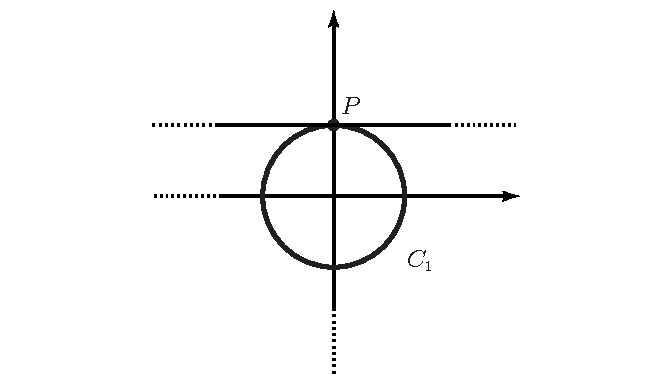
\includegraphics[trim=0cm 0cm 0cm 0cm,clip,scale=0.50]{images/planecurve1.pdf}
\end{minipage}
\end{example}
\begin{example} \label{esempiocurvaq}	Sia $C$ in $\aff{\realset^2}$ la curva di equazione $f\ \colon y^2=x^2+x^3=x^2(x+1)$, una \textbf{cubica} in quanto ha grado 3.\\
Vogliamo calcolare quali sono le rette tangenti nel punto $P=(-1,\ 0)\in C$. Consideriamo pertanto il fascio di rette passanti per $P$ e le intersechiamo con la cubica per determinare quali sono tangente con la definizione; guardiamo dunque quali hanno molteplicità di intersezione maggiore di 1.\\
Il fascio di rette per $P$ è:
\begin{equation*}
	r\colon \begin{cases}
		x=-1+tv_1\\
		y=tv_2
	\end{cases}
\end{equation*}
Con $(v_1,\ v_2)$ direzione di $r$. Sostituiamo la parametrizzazione di $r$ nell'equazione di $C$, costruendo la funzione $g\left(t\right)$:
	\begin{gather*}
		t^2v^2=(tv_1-1)^2 tv_1\\
		g(t)=(tv_1-1)^2tv_1-t^2v_2^2=t[v_1(t^2v_1^2+1-2tv_1)-tv_2^2]=t[v_1^3t^2-t(2v_1^2+v_2^2)+v_1]
	\end{gather*}
	Analizziamo cosa abbiamo trovato:
		\begin{itemize}
			\item $t=0$ è sempre una soluzione: per costruzione abbiamo preso la retta che passava per $P$, dunque $P$ è banalmente intersezione di una retta di \textit{qualsiasi} direzione con la cubica.
			\item La molteplicità di intersezione fra $C$ e $r$ in $P$ è la massima potenza di $t$ che divide $g$; pertanto è $m$ se $t^m$ è la massima potenza di $t$ che divide $g$.\\
			In questo caso, quand'è che la molteplicità di intersezione è maggiore di 1? Nell'equazione che abbiamo scritto almeno $t^2$ deve dividere $g$: l'unica possibilità per questa curva di poter raccogliere un'altro $t$ è avere $v_1=0$. Allora $r$ è la retta verticale che passa per $P$ e abbiamo determinato che esiste ed è l'\textit{unica} tangente in $P$.
		\end{itemize}
	Vediamo ora un caso in cui la retta tangente ad un punto non è unica. Consideriamo la stessa cubica ma \textit{cambiamo il punto}, prendendo l'origine $Q=\left(0,\ 0\right)\in C$.\\
	Scriviamo il fascio di rette per $Q$:
	\begin{equation*}
		q\colon \begin{cases}
			x=tw_1\\
			y=tw_2
		\end{cases}
	\end{equation*}
	Con $(w_1,\ w_2)$ direzione. Analogamente a prima:
	\begin{gather*}
		h(t)=t^2w_1^2+t^3w_1-t^2w_2^2=t^2(w_1^2-w_2^2+tw_1^3)
	\end{gather*}
\begin{minipage}{0.75\textwidth}
Troviamo così che $t^2$ si può sempre raccogliere, dunque in questo caso la molteplicità di intersezione fra le rette e $Q$ è sempre almeno 2. In particolare, ogni retta per $Q$ ha intersezione maggiore di 2, dunque è \textit{tangente}.\\
Osserviamo che nel punto $Q$ la curva si auto-interseca: ogni retta per l'origine interseca la curva almeno due volte, quindi è tangente. Fra queste, ci sono due \textit{direzioni speciali} per cui la molteplicità è 3:
\begin{itemize}
	\item $w_1^2-w_2^2=0\implies w_1=w_2 \implies \mathcal{L}(1,1) \colon y=x$.
	\item $w_1=-w_2 \implies \mathcal{L}(1,-1) \colon y=-x$.
\end{itemize}
\end{minipage}
\hspace{-12mm}
\begin{minipage}{0.24\textwidth}
	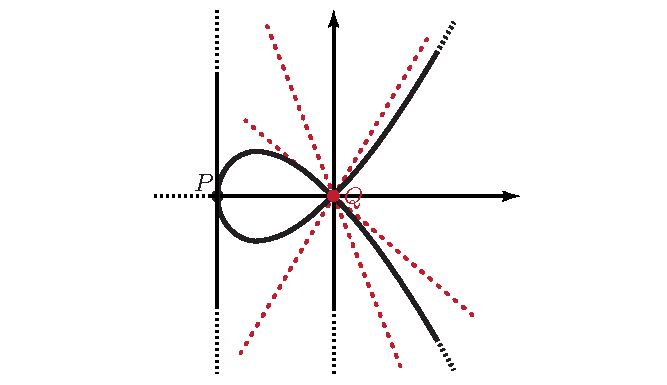
\includegraphics[trim=0cm 0cm 0cm 0cm,clip,scale=0.50]{images/planecurve2.pdf}
\end{minipage}
\end{example}
\subsubsection{Caso affine}
Sia $C\colon f\left(x,\ y\right)=0$ in $\kamp^2$ e $P=(x_0,\ y_0)$. Osserviamo che possiamo sempre scrivere il polinomio come un polinomio centrato in $x_0,\ y_0$, cioè come polinomio in $x-x_0$ e $y-y_0$ invece che come polinomio in $x$ e $y$.
\begin{gather*}
		f=\sum_{i,j\geq 0} a_{ij}x^iy^j = \sum_{i,j\geq 0} a_{ij}(x-x_0+x_0)^i(y-y_0+y_0)^j \stackrel{!}{=} 	\sum_{i,j\geq 0}b_{ij}(x-x_0)^i(y-y_0)^j\\
		\implies f(x_0,\ y_0)=b_{00}=f\left(P\right) \implies f=f\left(P\right) +\alpha (x-x_0)+\beta (y-y_0)+ \text{ termini di grado} >1
\end{gather*}
Nel passaggio indicato con (!) si stanno sottintendendo conti con il binomio di Newton.\\
\begin{define}[Derivate parziali.]~{}\\
	Dato un polinomio $f=\sum_{i,j}a_{ij}x^iy^j\in\kamp[x,\ y]$, le \textbf{derivate parziali}\index{derivata!parziale} di $f$ sono i seguenti polinomi:
	\begin{equation}
		\frac{\partial{f}}{\partial{x}}\coloneqq \sum_{i,j}a_{ij}ix^{i-1}y^j\quad \frac{\partial{f}}{\partial{y}}\coloneqq \sum_{i,j}a_{ij}jx^iy^{j-1}
	\end{equation}
\vspace{-3mm}
\end{define}
Si verifica che $\alpha=\frac{\partial{f}}{\partial{x}}(x_0,\ y_0)$ e $\beta=\frac{\partial{f}}{\partial{y}}(x_0,\ y_0)$.
\begin{demonstration}
	Se $P\in C$, segue dai ragionamenti precedenti $f=\alpha (x-x_0)+\beta (y-y_0)+ \text{ termini di grado} >1$. Applicando la definizione di derivata parziale si hanno:
	\begin{equation*}
		\frac{\partial{f}}{\partial{x}}= \sum_{i,j}a_{ij}i\left(x-x_0\right)^{i-1}\left(y-y_0\right)^j\quad \frac{\partial{f}}{\partial{y}}= \sum_{i,j}a_{ij}j\left(x-x_0\right)^i\left(y-y_0\right)^{j-1}
	\end{equation*}
	Valutando in $P=(x_0,\ y_0)$:
	\begin{equation*}
		\frac{\partial{f}}{\partial{x}}\left(P\right)=a_{10}=\alpha\quad \frac{\partial{f}}{\partial{y}}\left(P\right)=a_{01}=\beta
	\end{equation*}
\end{demonstration}
%LEZ 35
\begin{define}[Gradiente.]~{}\\
	Il \textbf{gradiente}\index{gradiente} $\nabla f$ è il vettore con componenti le derivate parziali:
	\begin{equation}
		\nabla f=\left( \frac{\partial{f}}{\partial{x}},\ \frac{\partial{f}}{\partial{y}} \right)
	\end{equation}
\vspace{-6mm}
\end{define}
Il gradiente valutato in $P=(x_0,\ y_0)$ è $\nabla f\left(P\right)=(\alpha,\beta)\in\kamp^2$.\\
%Adesso vogliamo intersecare con l retta genereica per P
\subsubsection{Tangente e derivate parziali}
Sia $r$ la retta per $P$ con direzione $v=(v_1,v_2)$ e descrizione parametrica:
\begin{equation*}
	\begin{cases}
		x=x_0+tv_1\\
		y=y_0+tv_2
	\end{cases}
\end{equation*}
Allora:
	\begin{equation*}
		\begin{array}{ll}
			g(t)=f(x_0+tv_1,\ y+tv_2)&=\alpha tv_1+\beta tv_2 + \text{ termini in }t\text{ di grado }\geq 2 =\\
			&= (\alpha v_1+\beta v_2)t + \text{ termini in }t \text{ di grado }\geq 2
		\end{array}	
	\end{equation*}
Si hanno dunque due possibilità, che dipendono dal coefficiente di $t$:
	\begin{enumerate}
		\item	$\alpha=\beta=0$, ovvero $\nabla f =0$: il \textit{coefficiente} è nullo indipendentemente dalla retta. Allora, $\forall r$ retta per $P$,  $t^2 \mid g(t)$: la molteplicità di intersezione è $\geq 2$ e \textit{ogni} retta per $P$ è tangente a $C$ in $P$.
		\item	$\nabla f\left(P\right)=(\alpha,\beta)\neq 0$:	il coefficiente di $t$ determina in maniera \textit{univoca} la direzione della retta, che è quella \textbf{ortogonale} a $(\alpha,\beta)$. Ciò implica che $\exists !$ retta tangente a $C$ in $P$ ed è quella di direzione $(-\beta,\alpha)$ con equazione	$\alpha(x-x_0)+\beta(y-y_0)=0$, ovvero
			\begin{equation}
				\frac{\partial{f}}{\partial{x}}\left(P\right)(x-x_0) + \frac{\partial{f}}{\partial{y}} \left(P\right)(y-y_0)=0
			\end{equation}
	\end{enumerate}
% Abbiamo così ritrovato la casistica della cubica con i punti espliciti: ogni retta è tangente oppure c'è una sola tangente alla curva nel punto.
\begin{define}[Punto singolare.]~{}\\
	Sia $C$ una curva affine in $\kamp^2$ di equazione $f\left(x,\ y\right)=0$. Un punto $P\in C$ è detto \textit{non singolare} o \textbf{liscio}\index{punto!liscio} se $\nabla f\left(P\right)\neq 0$. Altrimenti $P$ è detto \textbf{punto singolare} \index{punto!singolare}.\\
	Una curva $C$ è detta \textbf{singolare} se ha almeno un punto singolare, altrimenti è detta curva \textit{non singolare} o \textbf{liscia}.
\end{define}
Abbiamo visto prima che se $P$ è \textit{non singolare} esiste ed è unica la tangente a $C$ in $P$. Essa ha equazione	$\frac{\partial{f}}{\partial{x}}\left(P\right)(x-x_0) + \frac{\partial{f}}{\partial{y}} \left(P\right)(y-y_0)=0$ e, essendo non singolare, almeno uno dei due coefficienti non è nullo.\\
Se invece $P$ è \textit{singolare} allora ogni retta per $P$ è tangente a $C$ in $P$.
\subsubsection{Caso proiettivo}
Vogliamo analizzare la tangenza nel \textit{caso proiettivo}. Tuttavia, prima di trattare di punti singolare o tangenti, ci servirà una proprietà dei polinomi omogenei, detta \textbf{relazione di Eulero} sui polinomi omogenei. Essa vale per un qualsiasi \textit{numero di variabili} a coefficienti in un campo \textit{qualsiasi} e mette in relazione un polinomio omogeneo con sue derivate parziali, che per costruzione sono polinomi omogenei di un \textit{grado inferiore}.
\begin{theorema}[Relazione di Eulero.]~{}\\ \index{Relazione!di Eulero}
	Sia $F\in\kamp[x_0,\ \ldots,\ x_n]$ polinomio omogeneo di grado $m$ e le sue derivate parziali $\frac{\partial{f}}{\partial{x_i}}\in\kamp[x_0,\ \ldots,\ x_n]$, polinomio omogenei di grado $m-1$. Si ha che:
		\begin{equation}
			\sum_{i=0}^n x_i\frac{\partial{F}}{\partial{x_i}}=mF
		\end{equation}
	\vspace{-6mm}
\end{theorema}
Nella relazione appena annunciata notiamo che moltiplichiamo ciascuna derivata parziale per $x_i$. Ciò è necessario per la \textit{buona definizione} dell'equazione: siccome le derivate parziali sono omogenee di grado $m-1$, moltiplichiamo per $x_i$ affinché la somma sia omogenea di grado $m$ come il polinomio $F$.
\begin{demonstration}
	Basta mostrarlo per un monomio $G=\lambda x_0^{j_0}\cdots x_n^{j_n}$ con $j_0+\ldots+j_n=m,\ \lambda\in\kamp$. Scrivendone le derivate parziali rispetto ad una variabile e poi moltiplicando per $x_i$ sistemiamo l'esponente $i$-esimo:
		\begin{gather*}
			\frac{\partial{G}}{\partial{x_i}}=\lambda j_i x_0^{j_0}\ldots x_i^{j_{i-1}} \ldots x_n^{j_n} \implies  x_i \frac{\partial{G}}{\partial{x_i}}=\lambda j_i x_0^{j_0}\ldots x_i^{j_i} \ldots x_n^{j_n}\\
			\implies \sum_{i=0}^n x_i\frac{\partial{G}}{\partial{x_i}} = \sum_{i=0}^n \lambda j_i x_0^{j_0} \ldots x_n^{j_n}=\lambda x_0^{j_0}\ldots x_n^{j_n} \cdot \sum_{i=0}^n j_i =mG
		\end{gather*}
\end{demonstration}
%il monomio è sempre lo stesso perché si moltiplica per x_i
%monomio j e somma degli esponenti è esattamente di grado, dunque =mG
%sing e non sing rette tang per piane pro
\begin{proposition}[Retta tangente e derivate parziali.]~{}\\
	Sia $C$ in $\proj[2]{\ }$ una curva di equazione $F\left(x_0,\ x_1,\ x_2\right)=0$ con $F$ polinomio omogeneo di grado $d$ e $P\in C$. $P$ è \textit{non singolare} se e solo se almeno una delle derivate parziali di F non è nulla in $P$, cioè $\exists i\in\{0,1,2\}\colon \frac{\partial{F}}{\partial{x_i}}\left(P\right)\neq 0$.\\
%allo stesso mod del caso affine con le der in p
	In tal caso esiste ed è unica la retta tangente a $C$ in $P$ ed ha equazione:
		\begin{equation}
			\underbrace{\frac{\partial{F}}{\partial{x_0}}\left(P\right) }_{\in\kamp}x_0 + \underbrace{\frac{\partial{F}}{\partial{x_1}}\left(P\right) }_{\in\kamp}x_1 + \underbrace{\frac{\partial{F}}{\partial{x_2}}\left(P\right) }_{\in\kamp}x_2
		\end{equation}
	I cui coefficienti sono le derivate parziali di $F$ valutate in $P$.
\end{proposition}
\begin{demonstration}
	% Dobbiamo verificare che per la curva affine di cui $C$ è chiusura proiettiva (ottenuta deomogeneizzando rispetto a $x_0$) si ritrova la retta tangente affine.\\
	A meno di proiettività possiamo supporre che $P=(1\colon a\colon b)\in U_0=\{x_0\neq 0\}$, cioè che stia nella carta affine $U_0$ identificata a $\aff{\kamp^2}$: $P$ corrisponde a $\left(a,\ b\right)\in\aff{\kamp^2}$.\\
	Poniamo $f\left(x,\ y\right)\coloneqq F(1,\ x,\ y)$ e sia $C_0$ la curva in $\aff{\kamp^2}$ di equazione $f\left(x,\ y\right)=0$ per cui $C$ è la chiusura proiettiva. Mettiamo in relazione le derivate parziali di $f$ con quelle $F$ a partire dalla definizione stessa di $f$,
%	che ci dice che facendo la derivate parziali di $f$ rispetto a $x$ è la sessa di 	valutata in	come polinomio, idem y, ed è una relazione fra polinomi
	valutandole nel punto:
		\begin{gather*}
			\begin{cases}
				\frac{\partial{f}}{\partial{x}} = \frac{\partial{F}}{\partial{x_1}} (1,\ x,\ y)\\
				\frac{\partial{f}}{\partial{y}} = \frac{\partial{F}}{\partial{x_2}} (1,\ x,\ y)
			\end{cases}
			\implies \textcolor{green}{\circled{\ast}}\quad
			\begin{cases}
				\frac{\partial{f}}{\partial{x}}\left(a,\ b\right) = \frac{\partial{F}}{\partial{x_1}} \left(1,\ a,\ b\right)\\
				\frac{\partial{f}}{\partial{y}}\left(a,\ b\right) = \frac{\partial{F}}{\partial{x_2}} \left(1,\ a,\ b\right)
			\end{cases}
		\end{gather*}
	Valutiamo la relazione di Eulero sui polinomi omogenei in $\left(1,\ a,\ b\right)$:
		\begin{gather*}
			\frac{\partial{F}}{\partial{x_0}}\left(1,\ a,\ b\right) + a\frac{\partial{F}}{\partial{x_1}}\left(1,\ a,\ b\right) + b\frac{\partial{F}}{\partial{x_2}}\left(1,\ a,\ b\right)= dF\left(1,\ a,\ b\right)=0
		\end{gather*}
	Si ha $F\left(1,\ a,\ b\right)=0$ perché $P\in C$. Riusciamo così a esprimere la derivata parziale rispetto a $x_0$ in funzione delle altre due:
		\begin{gather*}
			\textcolor{green}{\circled{\ast\ast}}\quad \frac{\partial{F}}{\partial{x_0}}=-a\frac{\partial{F}}{\partial{x_1}} -b\frac{\partial{F}}{\partial{x_2}}
		\end{gather*}
	Ne consegue che $\nabla f\left(a,\ b\right)=0 \iff  \nabla F\left(1,\ a,\ b\right)=(0,0,0)$; infatti, se il gradiente $\nabla f$ si annulla in $P$ allora si annullano le derivate parziali di $F$ rispetto a $x_1,\ x_2$, pertanto per la relazione di Eulero anche la terza derivata parziale si annulla. Viceversa, se il gradiente di $F$ si annulla bastano le relazioni $\textcolor{green}{\circled{\ast}}$ per avere che anche il gradiente di $f$ si annulla.\\
	Dunque, il punto $P$ è \textit{non singolare} se e solo se $\nabla F\left(1,\ a,\ b\right)\neq \mathbf{0}$, verificando la prima parte della proposizione.\\
	Supponendo $P$ non singolare, allora la retta tangente affine a $C_0$ in $P$ ha equazione:
	\begin{equation*}
		\frac{\partial{f}}{\partial{x}}\left(a,\ b\right)(x-a) + \frac{\partial{f}}{\partial{y}}\left(a,\ b\right)(y-b)=0
	\end{equation*}
	La chiusura proiettiva di tale retta affine dà la retta tangente proiettiva a $C$ in $P$:
	\begin{equation*}
		\frac{\partial{f}}{\partial{x}}\left(a,\ b\right)(x_1-ax_0) + \frac{\partial{f}}{\partial{y}}\left(a,\ b\right)(x_2-bx_0)=0
	\end{equation*}
	Per $\textcolor{green}{\circled{\ast}}$ si ha che
		\begin{equation*}
			\begin{array}{ll}
				&\frac{\partial{F}}{\partial{x_1}}\left(1,\ a,\ b\right)(x_1-ax_0) + \frac{\partial{F}}{\partial{x_2}}\left(1,\ a,\ b\right)(x_2-bx_0)=0 \\[3mm]
				\implies & \underbrace{ \left( -a\frac{\partial{F}}{\partial{x_1}}\left(1,\ a,\ b\right) -b \frac{\partial{F}}{\partial{x_2}}\left(1,\ a,\ b\right) \right)}_{\textcolor{green}{\circled{\ast\ast}}}  x_0 + \frac{\partial{F}}{\partial{x_1}}\left(1,\ a,\ b\right) x_1 + \frac{\partial{F}}{\partial{x_2}}\left(1,\ a,\ b\right) x_2=0 \\
				\implies & \frac{\partial{F}}{\partial{x_0}}\left(P\right) x_0 + \frac{\partial{F}}{\partial{x_1}}\left(P\right) x_1 + \frac{\partial{F}}{\partial{x_2}}\left(P\right) x_2
			\end{array}
		\end{equation*}
\end{demonstration}

\begin{observe} \textsc{Rette tangenti: spazio affine e spazio proiettivo a confronto.}\\
	Se $C$ è una curva affine di equazione $f\left(x,\ y\right)=0$, per trovare i punti singolare di $C$ bisogna risolvere un sistema con l'equazione della curva e le derivate parziali di $f$. L'equazione della curva è necessaria perché potrei avere punti in cui il gradiente si annulla ma \textit{non} appartengono alla curva!\\
	Invece, se $C$ è una curva proiettiva di equazione $F\left(x_0,\ x_1,\ x_2\right)=0$, per trovare i punti singolari di $C$ bisogna solo risolvere il sistema delle derivate parziali nulle e \textit{non serve} mettere anche l'equazione della curva per via della relazione di Eulero. Infatti, se $P$ annulla $\nabla F$, allora dalla relazione di Eulero si ha che:
		\begin{equation*}
			F\left(P\right)=\frac{1}{d}\left( a\frac{\partial{F}}{\partial{x_0}}\left(P\right) + b\frac{\partial{F}}{\partial{x_1}}\left(P\right) + c\frac{\partial{F}}{\partial{x_2}}\left(P\right) \right) = 0 \implies P\in C
		\end{equation*}
	Riassumendo, ecco i sistemi a confronto:
		\begin{center}
			\begin{tabular}{c|c}
				Affine & Proiettivo \\
				\hline
				$\displaystyle \begin{cases}
					f\left(x,\ y\right)=0 \\		\frac{\partial{f}}{\partial{x}}\left(x,\ y\right)=0\\	\frac{\partial{f}}{\partial{y}}\left(x,\ y\right)=0
				\end{cases}$ & $\displaystyle \begin{cases}
					\frac{\partial{F}}{\partial{x_0}}=0\\	\frac{\partial{F}}{\partial{x_1}}=0\\	\frac{\partial{F}}{\partial{x_2}}=0
				\end{cases}$
			\end{tabular}
		\end{center}
\end{observe}

\begin{examples} \label{esempi lez 35}
	\begin{enumerate}
		\item	Sia $C_0\colon x^2+x^3-y^2=0$ una curva affine e $C$ la chiusura proiettiva di $C_0$ con equazione $F=x_0x_1^2+x_1^3-x_0x_2^2$. Cerchiamo i punti singolari:
			\begin{gather*}
				\nabla F=0 \iff \begin{cases}
					\frac{\partial{F}}{\partial{x_0}}=x_1^2 - x_1^2=0\\
					\frac{\partial{F}}{\partial{x_1}}=2x_0x_1+3x_1^2=0\\
					\frac{\partial{F}}{\partial{x_2}}-2x_0x_2=0
				\end{cases} \implies \begin{cases}
					x_0=0 \\ x_1=0 \\ x_2=0
				\end{cases} \text{ oppure } \begin{cases}
					x_0=t \\ x_1=0 \\ x_2=0
				\end{cases}
			\end{gather*}
		Il primo non è lecito nel piano proiettivo, dunque $P=(1\colon 0\colon 0)$ è l'unico punto singolare di $C$ e osserviamo che corrisponde a $(0,\ 0)\in\kamp^2$.\\
		A pagina \pageref{esempiocurvaq} avevamo visto il punto $Q=(-1,\ 0)\in C_0$, nel quale la curva affine si auto-intersecava; passando alla chiusura proiettiva, $Q=(1\colon -1\colon 0)\in C$ è \textit{non} singolare. Scriviamo la tangente $T_Q C$ grazie alle derivate parziali:
		\begin{equation*}
			\frac{\partial{F}}{\partial{x_0}}\left(Q\right)=1,\ \frac{\partial{F}}{\partial{x_1}}\left(Q\right)=(2x_0x_1+3x_1^2)\left(Q\right)=1,\ \frac{\partial{F}}{\partial{x_2}}\left(Q\right)=(-2x_0x_1)\left(Q\right)=0
		\end{equation*}
		Ne segue che $T_Q C\colon x_0+x_1=0$. Per ottenere la retta affine associata basta porre $x_0=1$, da cui $T_Q C_0\colon x+1=0$, perfettamente coerente con lo studio fatto nel caso affine.\\
		Avevamo visto che nel punto singolare $P=(1\colon 0\colon 0)$, tutte le rette per esso hanno molteplicità di intersezione $2$ con la curva $C$ in $P$, eccetto due rette speciali di direzione $(1,\ \pm 1)$ in cui la molteplicità di intersezione è 3. $P$ è detto \textbf{nodo}.
		\item	Consideriamo la curva affine $C_0$ data da $f\left(x,\ y\right)=y^2-x^3$ e la chiusura proiettiva $C$ di equazione $F(x_0,\ x_1,\ x_2)=x_0x_2^2-x_1^3$. Siccome:
		\begin{equation*}
			\frac{\partial{F}}{\partial{x_0}} =x_2^2,\ \frac{\partial{F}}{\partial{x_1}}= -3x_1^2,\ \frac{\partial{F}}{\partial{x_2}}= 2x_0x_2
		\end{equation*}
		Allora $P=(1\colon 0\colon 0)$ è l'unico punto singolare di $C$, che corrisponde all'origine di $\aff{\kamp^2}$. Consideriamo il fascio di rette per l'origine in $\aff{\kamp^2}$ e vediamo qual è la molteplicità di intersezione. Sia la generica retta per l'origine:
		\begin{equation*}
			r\colon \begin{cases}
				x=tv_1 \\
				y=tv_2
			\end{cases}\text{ con } v=(v_1,\ v_2)\text{ direzione di }r
		\end{equation*}
		La intersechiamo con $C_0$:
		\begin{equation*}
			g(t)=t^2v_2^2 -t^3v_1^3=0 \implies t^2(v_2^2 -tv_1^3)=0
		\end{equation*}
		Segue che la molteplicità di intersezione in $P$ è 2 se $v_2\neq 0$ ed è 3 se $v_2=0$.
		\begin{minipage}{0.65\textwidth}
			Si noti che i risultati ottenuti sono simili al caso precedente: la differenza sta nel fatto che quasi tutte le rette hanno molteplicità 2 e c'è solo un'unica retta con molteplicità 3 e non \textit{due} come nel caso precedente.\\
			Disegnando la curva affine si nota dunque la presenza di una \textbf{cuspide}.
		\end{minipage}
		\hspace{-12mm}
		\begin{minipage}{0.34\textwidth}
			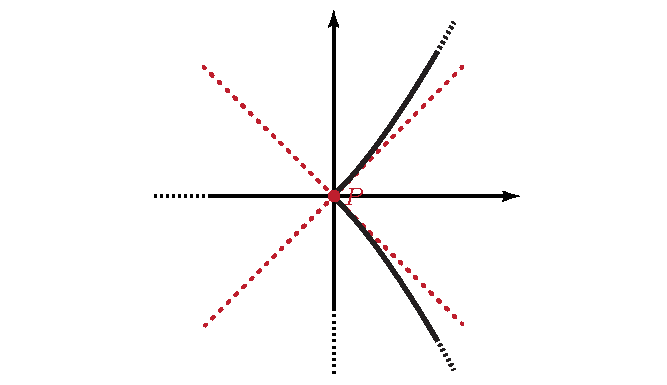
\includegraphics[trim=0cm 0cm 0cm 0cm,clip,scale=0.50]{images/planecurve3.pdf}
		\end{minipage}
	\end{enumerate}
\end{examples}
\begin{observe} \textsc{Punti singolari delle coniche.}\\
	Sia $C$ una conica proiettiva. Il \textit{numero} di punti singolari dipende solo dal \textit{rango}:
		\begin{itemize}
			\item	$\rk C=3\implies C$ \textit{non} ha punti singolari.
			\item	$\rk C=2 \implies C$ ha \textit{un} punto singolare.
			\item	$\rk C=1 \implies C$ è una \textit{retta doppia} e \textit{ogni punto} di $C$ è singolare.
		\end{itemize}
	Infatti, sia $A$ la matrice simmetrica associata a $C$, allora l'equazione associata a $C$ e le derivate parziali sono:
		\begin{gather*}
			F=X^tAX=\sum_{i,j=0}^2 a_{ij}x_ix_j \implies \frac{\partial{F}}{\partial{x_h}} = \sum_{\stackrel{j=0}{\left(i=h\right)}}^2 a_{hj}x_j+ \sum_{\stackrel{i=0}{\left(j=h\right)}}^2  a_{ih}x_i = 2\sum_{i=0}^2 a_{ih}x_i
		\end{gather*}
	Un punto $P$ rappresentato dal vettore $v$, ovvero $P=[v]$, è singolare per $C$ se le derivate parziali si annullano, cioè se $\displaystyle\sum_{i=0}^2 a_{hi}v_i=\sum_{i=0}^2 a_{ih}v_i=0,\ \forall h=0,1,2$. In \textit{notazione matriciale}, se si pensa al prodotto righe per colonne l'indice di riga di $a$ è fissato in $h$ mentre facciamo variare l'indice di colonna $i$. Se $v=\begin{psmallmatrix} v_0 \\ v_1 \\ v_2 \end{psmallmatrix}$ è il vettore, porre l'$h$-esima riga di $Av$ pari a zero è proprio la condizione cercata $\displaystyle\sum_{i=0}^2 a_{ih}v_i$. Ne segue che avere il gradiente nullo corrisponde a $Av=0$, cioè $v\in\ker A$.\\
	Riassumendo, i punti singolari di $C$ sono dati dai vettori che stanno nel nucleo della matrice $A$, che dipende dal rango di $A$:
		\begin{itemize}
			\item	$\rk A=3\implies \ker A=\{0 \} \implies C$ \textit{non} ha punto singolare.
			\item	$\rk A=2\implies \dim\ker A=1 \implies C$ ha \textit{un} punto singolare.
			\item	$\rk A=1\implies F=\lambda L^2 \implies C$ è una \textit{retta doppia} e \textit{ogni punto} di $C$ è singolare; è esattamente la retta proiettiva associata al nucleo di $A$: $L=\mathbb{P}(\ker A)$.
		\end{itemize}
\begin{minipage}{0.75\textwidth}
Analizziamo il caso $\rk C=2$ rispetto alla classificazione delle coniche.\\
Se $\kamp=\complexset$, $C=L_1\cup L_2$ con $L_1\neq L_2$ distinte e il punto singolare è il punto di \textit{intersezione} delle due rette, ovvero $L_1\cap L_2$.
Se $\kamp=\realset$, a meno di proiettività si hanno 2 casi in base alla segnatura:
	\end{minipage}
	\hspace{-12mm}
	\begin{minipage}{0.24\textwidth}
		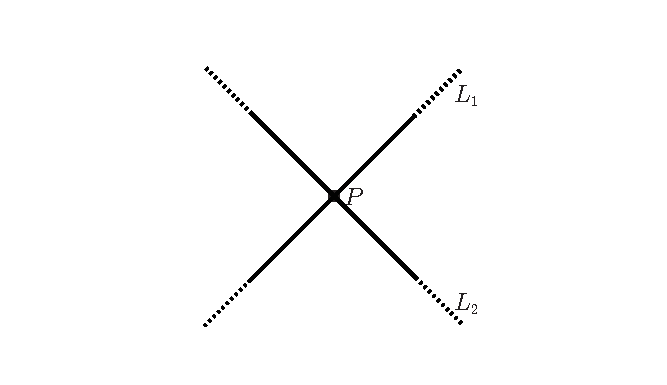
\includegraphics[trim=0cm 0cm 0cm 0cm,clip,scale=0.50]{images/planecurve4.pdf}
	\end{minipage}
\begin{itemize}
	\item $(1,1)$: $C=L_1\cup L_2$ e $P=L_1\cap L_2$.
	\item $(2,0)/(0,2)$: La forma quadratica si fattorizza su $\complexset$ e non su $\realset$; $C$ ha come sostegno un \textit{unico} punto $P$, che è proprio il punto singolare.
\end{itemize}
\end{observe}
\begin{observe}\textsc{Punti singolari e cubiche.}\\
	Nel piano proiettivo $\proj[2]{\kamp}$ consideriamo $C$ una \textit{cubica} di equazione $F=0$ con $\deg F=3$. Se la curva $C$ è \textit{riducibile}, allora il polinomio $F$ è \textit{riducibile} per definizione, ma siccome il grado è solo 3, allora è necessariamente il prodotto di un polinomio di grado 1 per un altro polinomio di grado 2:
	\begin{equation*}
		F=G\cdot H\text{ con }\deg G=1\text{ e }\deg H=2
	\end{equation*}
	Il luogo degli zeri di $F$ è \textit{unione} dei luoghi degli zeri di $G$ e $H$, dunque $C$ è unione di una retta e di una conica.\\ \hspace{-1mm}
	\begin{minipage}{0.75\textwidth}
	\vspace{2mm}
	Supponiamo invece che $C$ sia \textit{irriducibile}: $C$ \textit{non} può contenere una retta, altrimenti l'equazione della retta \textit{dividerebbe} il polinomio $F$. Allora $C$ ha \textit{al più un punto singolare}.
	Supponiamo per assurdo ne abbia almeno due, come $P$ e $Q$: potremmo considerare la retta $r=\overline{PQ}$ che passa per $P$ e $Q$ e intersecarla con la curva. Sicuramente $C\cap r\supseteq \{P,Q\}$ e, siccome $P$ e $Q$ sono due punti singolari, allora la molteplicità di intersezione è almeno 2.
	\end{minipage}
	\hspace{-12mm}
	\begin{minipage}{0.24\textwidth}
		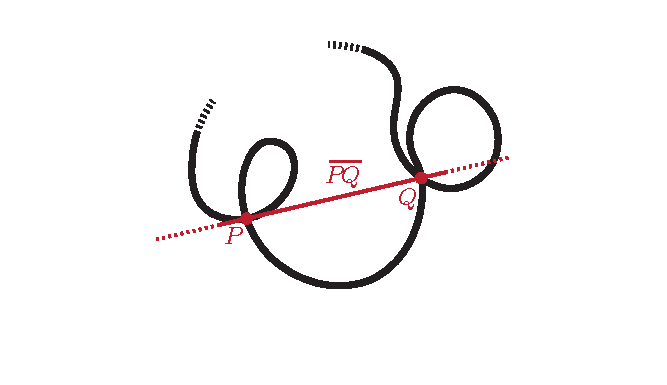
\includegraphics[trim=0cm 0cm 0cm 0cm,clip,scale=0.50]{images/planecurve5.pdf}
	\end{minipage}\\
	Ma ciò non è possibile perché, dallo studio delle intersezioni fra una retta e una curva, sappiamo che dobbiamo contare con molteplicità \textit{fino al grado della curva}: qui ci sono $2$ punti con molteplicità $2$, ma $C$ ha grado 3, dunque la retta dovrebbe essere contenuta nella curva, il che è una contraddizione!
\end{observe}
\begin{example}
	Sia $F=x_0^3+x_1^3+x_2^3$. Essa dà una curva \textit{senza punti singolari} perché le derivate parziali sono multipli delle coordinate, dunque non possono mai essere tutti nulli
\end{example}
\section{Fasci di coniche proiettive}
\begin{define}[Fascio di coniche.]~{}\\
Siano $C_1$ e $C_2$ due coniche \textit{distinte} nel piano proiettivo $\proj[2]{\ }$ di equazioni $F_1$ e $F_2$, dunque con $F_1$ e $F_2$ sono proporzionali. Il \textbf{fascio di coniche}\index{fascio!di coniche} $\mathcal{F}$ generato da $C_1$ e da $C_2$ è dato da tutte le coniche di equazione:
\begin{equation}
	C_{\lambda,\mu}\colon \lambda F_1+\mu F_2=0\text{ con }(\lambda\colon \mu)\in \proj[1]{\ }
\end{equation}
\vspace{-6mm}
\end{define}
Notiamo che se moltiplichiamo $\lambda$ e $\mu$ per lo stesso scalare tutta l'equazione viene moltiplicata per lo stesso scalare, riottenendo la stessa conica di prima; $\lambda$ e $\mu$ vanno presi in $\proj[1]{\ }$ e non solo in $\kamp$.
\begin{examples}
	\begin{enumerate}
		\item	Siano $C_1\colon x_0x_1=0$ e $C_2\colon (x_0-x_1)x_2=0$ due coniche, entrambe coppie di rette. Il fascio da loro generato è $C_{\lambda,\mu}\colon \lambda x_0x_1 + \mu (x_0-x_1)x_2=\lambda x_0x_1 + \mu x_0x_2 -\mu x_1x_2=0$.
		\item	Siano $C_1\colon x_0x_1=0$ e $\widetilde{C_2}\colon x_0x_2=0$ due coniche. Il fascio da loro generato è $C_{\lambda,\mu}\colon \lambda x_0x_1 +\mu x_0x_2=x_0(\lambda x_1 + \mu x_2)=0$; siccome $x_0=0$ appartiene ad entrambe le coniche si può raccogliere.
	\end{enumerate}
\vspace{-3mm}
\end{examples}
Dato un fascio di coniche ci si chiede qual è il rango delle coniche del fascio.
\begin{define}[Conica degenere.]~{}\\
Una conica $C$ in $\proj[2]{\ }$ si dice \textbf{degenere}\index{conica!degenere} quando \textit{non} ha rango massimo, ovvero se $\rk C< 3$, dunque quando la matrice non è invertibile.
\end{define}
\begin{digression}
	 Si può dimostrare che il rango della conica,  ‘‘essere riducibili'' e ‘‘essere degeneri'' sono tutte proprietà proiettive. Dalla classificazione delle coniche proiettive (reali o complesse) si vede dunque che una conica è \textit{degenere} se e solo se è \textit{riducibile}.
\end{digression}
\subsection{Studio delle coniche degeneri di un fascio}
Dato un fascio, vogliamo vedere quante e quali sono le coniche degeneri del fascio. Supponiamo che $C_1$ abbia matrice simmetrica associata $A_1$ e $C_2$ abbiamo analogamente $A_2$. È chiaro che la conica del fascio $C_{\lambda,\mu}$ generata da $C_1,\ C_2$ sarà associata alla combinazione lineare $\lambda A_1+\mu A_2$ delle matrici: essa è una matrice $3\times 3$ i cui elementi sono o $0$ o forme lineari in $\lambda$ e $\mu$.\\
Definiamo $D(\lambda,\mu)\coloneqq \det (\lambda A_1+\mu A_2)$, polinomio omogeneo in $\lambda$ e $\mu$. Si hanno due possibilità:
	\begin{itemize}
		\item	$D(\lambda,\ \mu)\equiv 0\implies$ \textit{tutte} le coniche del fascio sono degeneri.
		\item	$D(\lambda,\ \mu)$ è omogeneo di grado 3, dunque le	coniche degeneri corrispondono agli \textit{zeri} del polinomio $D$ su $\proj[1]{\ }$. Poiché essi sono al più 3, ci sono \textit{al più 3 coniche degeneri}.
	\end{itemize}
\begin{tips}
	O tutte le coniche del fascio sono degeneri o sono al massimo 3, quindi se in un fascio ne trovo \textit{quattro} degeneri, allora tutte lo sono!
\end{tips}
Nel \textit{caso complesso} gli zeri (contati con molteplicità) sono pari al grado, dunque si ha sempre almeno una conica degenere. Lo stesso vale anche nel caso reale, essendo il grado del polinomio dispari.
Ristudiamo con quest'ottica gli esempi precedenti.
\begin{examples}
	\begin{enumerate}
		\item	Il fascio è $\mathcal{F}_1\colon 2(\lambda x_0x_1 +\mu x_0x_2 -\mu x_1x_2)=0$ ed ha matrice $A_{\lambda,\mu}=\begin{pmatrix}
			0 & \lambda & \mu \\
			\lambda & 0 & -\mu \\
			\mu & -\mu & 0
		\end{pmatrix}$. Pertanto $D(\lambda,\mu)=\det A_{\lambda,\mu}=-\lambda(\mu^2)+\mu(-\lambda \mu)=-2\lambda\mu^2$. Ci sono solo due zeri di cui uno doppio: $(\lambda\colon\mu)=(1\colon 0)$ oppure $(0\colon 1)$. Questi valori dei parametri ci restituiscono i polinomi di partenza, corrispondono dunque a $C_1$ e $C_2$, che sapevamo già essere degeneri in quanto coppie di rette. Abbiamo dunque scoperto che $C_1$ e $C_2$ sono le \textit{uniche coniche degeneri} del fascio.
		\item	Il fascio è $\mathcal{F}_2 \colon x_0(\lambda x_1+\mu x_2)=0$. In questo caso il determinante viene identicamente nullo $\left(D\equiv 0\right)$. In questo fascio tutte le coniche hanno una retta in comune.
	\end{enumerate}
\end{examples}

\begin{define}[Punti base di un fascio di coniche.]~{}\\
	I \textbf{punti base}\index{punti!base} di un fascio di coniche sono i punti che appartengono a \textit{tutte} le coniche del fascio:
		\begin{equation}
			\{\text{punti base}\}=\inter_{C\in\mathcal{F}} C \subset \proj[2]{\ }
		\end{equation}
	\vspace{-3mm}
\end{define}
\begin{observe}	I punti base di un fascio sono dati dall'intersezione delle due coniche che generano il fascio, cioè $C_1\cap C_2$. Infatti, $\displaystyle C_1\cap C_2 \supseteq \inter_{C\in\mathcal{F}} C$. Viceversa se $P\in C_1\cap C_2$ allora:
	\begin{equation*}
		F_1\left(P\right)=0\text{ e }F_2\left(P\right)=0 \implies (\lambda F_1 +\mu F_2)\left(P\right)=0,\ \forall\lambda,\mu \implies P\in C_{\lambda,\mu},\ \forall (\lambda\colon\mu)\in\proj[1]{\ }
	\end{equation*}
Dunque, per ogni qualunque combinazione lineare presa in $P$ si annulla, dunque $P$ è punto comune a tutte le coniche del fascio, cioè un punto base.
\end{observe}
Vediamo i punti base degli esempi precedenti.
\begin{examples}
	\begin{enumerate}
		\item	Per ottenere i punti base del fascio si intersecano le coniche che lo generano:
			\begin{gather*}
				\begin{cases}
					x_0x_1=0\\
					(x_0-x_1)x_2=0
				\end{cases} \implies \begin{cases}
					x_0=x_1=0\\
					x_0=x_2=0\\
					x_1=x_2=0
				\end{cases}
			\end{gather*}
		Intersecando due rette \textit{non} coincidenti si possono ottenere al più 4 punti, ma se ne ottengono meno se qualcuno di questi punti coincide con altri. In questo caso si hanno 3 punti base: $(1\colon 0\colon 0),(0\colon 1\colon 0), (0\colon 0\colon 1)$.
		\item	I punti base sono dati dal sistema:
		\begin{equation*}
			\begin{cases} x_0x_1=0\\ x_0x_2=0 \end{cases}
		\end{equation*}
		$x_0=0$ è una retta appartenente a \textit{tutte} le coniche del fascio, dunque si ha una \textit{retta di punti base}. L'altro punto base è $P=(1\colon 0\colon 0)$; notiamo che quest'ultimo è il punto base del fascio di rette $\lambda x_1+\mu x_2=0$, cioè il fascio di rette che contengono $P$.
	\end{enumerate}
\end{examples}
\begin{digression} \textsc{Nodi e Cuspidi}\\
	Un \textbf{nodo}\index{nodo} è un punto $P$ per cui la retta ‘‘generale'' per $P$ ha intersezione $2$ con la curva e ce ne sono \textit{esattamente} $2$ che hanno intersezione $>2$.\\
	Una \textbf{cuspide}\index{cuspide} è un punto $P$ in cui la retta ‘‘generale'' per $P$ ha intersezione $2$ con la curva e ce n'è \textit{una sola} che ha intersezione $>2$
\end{digression}
%LEZ 36
\section{Parametrizzazione delle coniche nel piano proiettivo}
Data l'equazione generale di una conica $F=a_{00}x_0^2+2a_{01}x_0x_1+\dots+a_{22}x_2^2$ possiamo associare a $C$ il punto $(a_{00}\colon a_{01}\colon a_{02}\colon a_{11}\colon a_{12}\colon a_{22})\in\proj[5]{\ }$, in quanto servono sei coordinate per descrivere una conica. Tale punto la determina univocamente: entrambi sono \textit{non} nulli e determinati \textit{a meno di multipli}.\\
In questo modo otteniamo una \textit{corrispondenza biunivoca} fra le coniche in $\proj[2]{\ }$ e $\proj[5]{\ }$:
	% https://q.uiver.app/?q=WzAsMixbMCwwLCJcXHtcXHRleHR7Y29uaWNoZSBpbiB9XFxwcm9qWzJde1xcIH0gXFx9Il0sWzIsMCwiXFxwcm9qWzVde1xcIH0iXSxbMCwxLCIxXFxjb2xvbiAxIiwwLHsic3R5bGUiOnsidGFpbCI6eyJuYW1lIjoiYXJyb3doZWFkIn19fV1d
	\[\begin{tikzcd}
		{\{\text{coniche in }\proj[2]{\ } \}} && {\proj[5]{\ }}
		\arrow["{1\colon 1}", from=1-1, to=1-3, tail reversed]
	\end{tikzcd}\]
Con questa interpretazione, cosa corrisponde un fascio di coniche?\\
Date $C_1$ e $C_2$ coniche, consideriamo il fascio $\mathcal{F}$ da loro generato: a $C_1\colon F=\sum_{i,j}a_{ij}x_ix_j$ corrisponde ad un punto $A=(a_{00}\colon \cdots \colon a_{22})\in\proj[5]{\ }$ e a $C_2\colon G=\sum_{i,j}b_{ij}x_ix_j$ corrisponde un punto $B=(b_{00}\colon\cdots\colon b_{22})\in\proj[5]{\ }$. La conica $C_{\lambda,\mu}$ del fascio è la combinazione lineare di $F$ e $G$, dunque i coefficienti dei monomi sono la combinazione lineare dei coefficienti delle equazioni di $C_1$ e $C_2$:
	\begin{gather*}
		c_{\lambda,\mu}\colon \lambda F+\mu G=\sum_{i,j}(\lambda a_{ij}+\mu b_{ij})x_ix_j \longleftrightarrow P_{\lambda,\mu} =(\lambda a_{00}+\mu b_{00}\colon \cdots \colon \lambda a_{22}+\mu b_{22})\in\proj[5]{\ }
	\end{gather*}
A $C_{\lambda,\mu}$ associamo il punto $P_{\lambda,\mu}$, le cui coordinate omogenee sono combinazioni lineari di $A$ e $B$. Facendo variare $\lambda$ e $\mu$, il punto $P_{\lambda,\mu}$ descrive in $\proj[5]{\ }$ una retta $\overline{AB}$ generata dai punti $A$ e $B$, pertanto \textit{un fascio di coniche corrisponde esattamente ad una retta in} $\proj[5]{\ }$. Siccome una retta è individuata da due qualsiasi suoi punti, allo stesso modo il fascio è descritto da qualsiasi sue due coniche, pertanto la scelta delle coniche dà solo una \textit{parametrizzazione diversa} del fascio.\\
Questo ci permette di dare alcune informazioni aggiuntive sui punti base:
\begin{tips} \textsc{Calcolo dei punti base con due coniche qualsiasi}.\\
	Dato un fascio $\mathcal{F}$ di coniche, i punti base del fascio sono dati dall'intersezione di \textit{due qualsiasi coniche} del fascio purché siano \textit{distinte}, ovvero da $C\cap\widetilde{C}$ dove $C$ e $\widetilde{C}$ sono due coniche distinte del fascio.
\end{tips}
%così è molto più facile intersecare coppie di rette
\begin{observe}
	Sia $\mathcal{F}$ un fascio di coniche. Esiste \textit{sempre} una conica $C$ degenere in $\mathcal{F}$, quindi usiamo $C$ per calcolare i punti base.\\
	Siccome è degenere, $C$ è l'unione di due rette linearmente indipendenti: $C=l_1\cup l_2$. Scegliamo una qualsiasi altra conica $\widetilde{C}$ del fascio; i punti base del fascio sono dati da $C\cap\widetilde{C}=(l_1\cap\widetilde{C})\cup (l_2\cap \widetilde{C})$.\\
	Ne deduciamo che il numero di punti base di un fascio di coniche, se sono finiti, sono 4: infatti, ciascuna delle due rette interseca $\widetilde{C}$ al più in 2 punti.
\end{observe}

\begin{corollary}[Intersezione di due coniche.]~{}\\
	Se due coniche $C_1$ e $C_2$ \textit{non} hanno una retta in comune allora:
	\begin{equation}
		\#(C_1\cap C_2)\leq 4
	\end{equation}
\vspace{-6mm}
\end{corollary}
\begin{demonstration}
	$C_1\cap C_2$ sono i punti base del fascio generato da $C_1$ e $C_2$. La tesi segue dall'osservazione precedente.
\end{demonstration}

\begin{tips} \textsc{Calcolo dell'intersezione delle coniche}.\\
	Abbiamo così anche un metodo per calcolare $C_1\cap C_2$ dato il fascio $\mathcal{F}$. Scriviamo $D(\lambda,\ \mu)$, troviamo una conica degenere $\widetilde{C}$ e poi intersechiamo con $C_1\cap\widetilde{C}$. Questo metodo è particolarmente utile nel caso avessimo a che fare con \textit{coniche irriducibili}.
\end{tips}
Ci sono diversi tipi di \textit{rappresentazione geometrica} dei fasci di coniche proiettive; vediamo quello più comune.
\begin{proposition}[Fascio di coniche per 4 punti in posizione generale.]~{}\\
	Siano $A,\ B,\ C,\ D$ quattro punti in posizione generale in $\proj[2]{\ }$.\\
	\begin{minipage}{0.75\textwidth}
	La famiglia delle coniche passanti per i quattro punti è un fascio $\mathcal{F}$ avente come punti base esattamente i quattro punti; geometricamente stiamo fissando $A,\ B,\ C,\ D$ e considerando le coniche che passano per tutti e quattro.\\
	Inoltre $\mathcal{F}$ non contiene rette doppie e contiene esattamente 3 coniche degeneri: esse sono le coppie di rette che
	passano per questi 4 punti: $\overline{AB}\cup\overline{CD}$, $\overline{AC}\cup \overline{BD}$, $\overline{AD}\cup\overline{BC}$.
	\end{minipage}
	\hspace{1mm}
	\begin{minipage}{0.24\textwidth}
		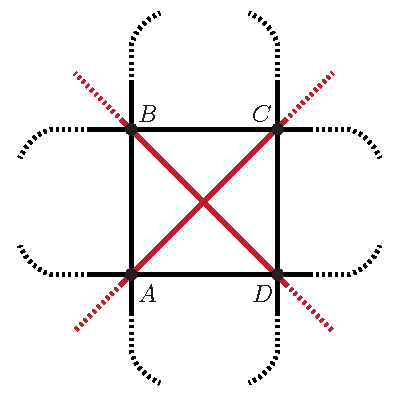
\includegraphics[trim=0cm 0cm 0cm 0cm,clip,scale=0.50]{images/conicfamily.pdf}
	\end{minipage}

%\footnote{il disegno è fuorviante perché le rette si intersecano da qualche parte nel piano proiettivo}
	
%famiglia fascio F: se la consider ocome punti di P5 descrivono esataente una retta: fissate due coniche le altre sono date da cl delle altre 2
%essere un fascio: in P5 è una retta: se guardo le eq tutte e sole che si ottengono come cl di due eq fissate/
%/è un fascio semplice perché il comportamento è quello che uno si aspetta/
\end{proposition}
\begin{demonstration}
	Siccome i 4 punti sono in posizione generale possiamo scegliere delle coordinate in $\proj[2]{\ }$ tali che i primi 3 sono i punti fondamentali e l'ultimo il punto unità: $A=(1\colon0\colon0), B=(0\colon1\colon0),\ C=(0\colon0\colon1),\ D=(1\colon1\colon1)$.\\
	Partiamo dall'equazione di una conica generica e imponiamo che passi per i 4 punti e vediamo le condizioni risultanti sui coefficienti:
		\begin{gather*}
			a_{00}x_0^2+2a_{01}x_0x_1+a_{11}x_1^2+2a_{02}x_0x_2+2a_{12}x_1x_2+a_{22}x_2^2=0\\
			\begin{array}{ll}
				\text{Per } A \colon & a_{00}=0 \\
				\text{Per } B \colon & a_{11}=0 \\
				\text{Per } C \colon & a_{22}=0 \\
				\text{Per } D \colon & 2a_{01}+2a{02}+2a_{12}=0 \implies a_{12}=-a_{01}-a_{02}
			\end{array}\\
			\implies a_{01}x_0x_1+a_{02}x_0x_2-(a_{01}+a_{02})x_1x_2=0
		\end{gather*}
	Abbiamo così le equazioni di tutte e sole le coniche che passano per $A,\ B,\ C,\ D$. Siccome $a_{01}$ e $a_{02}$ sono gli unici parametri rimasti, riscriviamo l'equazione evidenziandoli: $a_{01}x_1(x_0-x_2)+a_{02}x_2(x_0-x_1)=0$. Abbiamo così trovato esattamente un fascio di coniche generato dalle due coniche entrambe degeneri:
		\begin{equation*}
			C_1\colon \underbrace{x_1}_{\overline{AC}} \underbrace{(x_0-x_2)}_{\overline{BD}}=0 \quad
			C_2\colon \underbrace{x_2}_{\overline{AB}} \underbrace{(x_0-x_1)}_{\overline{CD}}=0
		\end{equation*}
	Abbiamo così dimostrato la prima affermazione.\\
	In questo modo abbiamo già trovato due coniche fra quelle degeneri del fascio; possiamo verificare, intersecando le due coniche (e quindi le quattro rette), che i punti base sono solo $A,\ B,\ C,\ D$:
	% Osserviamo ora che i punti base con coordinata $x_1$ zero sono proprio $A$ e $C$, pertanto $x_1=0$ corrisponde alla retta $\overline{AC}$. In modo analogo $x_2=0$ corrisponde alla retta $\overline{AB}$.
		\begin{equation*}
			\begin{array}{ll}
				C_1\cap C_2  & = (\overline{AC}\cup \overline{BD}) \cap (\overline{AB}\cup\overline{CD}) =\\ =(\overline{AC}\cap\overline{AB}) \cup (\overline{AC}\cap\overline{CD}) \cup (\overline{BD}\cap \overline{AB}) \cup (\overline{BD}\cap \overline{CD})=\\
				&=\{A,\ B,\ C,\ D\}
			\end{array}
		\end{equation*}
	Avremmo potuto evitare questo conto osservando che sono punti base perché per costruzione tutte le coniche passano per questi 4 punti e, essendo finiti, non possono essercene altri.\\
	Per trovare l'ultima conica degenere scriviamo la matrice associata a meno di multipli alla conica generica del fascio e calcoliamo le radici del suo determinante:
		\begin{gather*}
			M=\begin{pmatrix}
				0 & a_{01} & a_{02} \\
				a_{01} & 0 & -a_{01}-a_{02}\\
				a_{02} & -a_{01}-a{02} & 0
			\end{pmatrix}\\
		\implies D=\det M= -a_{01}a_{02}(a_{01}+a_{02})+a_{02}a_{01}(-a_{01}-a_{02}) = -2a_{01}a_{02}(a_{01}+a_{02})
		\end{gather*}
	È un polinomio omogeneo in $a_{01}$ e $a_{02}$ già fattorizzato in fattori lineari, pertanto si hanno esattamente \textit{tre} coniche degeneri: $a_{01}=0$ dà $C_2$, $a_{02}=0$ dà $C_1$, mentre la terza si ottiene sostituendo nell'equazione del fascio $a_{02}=-a_{01}$, da cui si ha l'equazione $a_{01}x_0x_1-a_{01}x_0x_2=0\implies x_0(x_1-x_2)=0$, corrispondente alle rette $\overline{BC}$ e $\overline{AD}$. Tutte e tre le coniche degeneri hanno rango 2 e quindi \textit{non} ci sono rette doppie nel fascio.
\end{demonstration}

\begin{tips} \textsc{Fascio di coniche per quattro punti in posizione generale}. \label{fascio coniche per 4 pt pos gen} \\
	Se dobbiamo scrivere un fascio $\mathcal{F}$ di coniche per quattro punti procedere come nella dimostrazione può esser lungo; in modo più rapido, scriviamo due delle coniche riducibili con delle rette per i punti:
	\begin{equation*}
		l_1\colon\overline{AB},\ l_2\colon \overline{CD},\ l_3\colon\overline{AC}, l_4\colon \overline{BD}
	\end{equation*}
	Le coniche sono $C_1\colon l_1l_2$ e $C_2\colon l_3l_4$; allora l'equazione del fascio è $\mathcal{F}\colon \lambda l_1 l_2 + \mu l_3 l_4 =0$.
\end{tips}
Se un punto di $\proj[2]{\ }$ è un punto base di un fascio, allora appartiene a tutte le coniche di esso. Preso invece un punto \textit{non} base del fascio, quante coniche passano per esso?
\begin{proposition}[Unicità della conica del fascio per il punto base.]~{}\\
	Sia $\mathcal{F}$ un fascio di coniche e sia $P\in \proj[2]{\ }$. Se $P$ \textit{non} è un punto base di $\mathcal{F}$, allora esiste ed è unica la conica del fascio che contiene $P$.
\end{proposition}
\begin{demonstration}
	Supponiamo di avere due coniche $C_1,\ C_2$ che generano il fascio $\mathcal{F}$ con $C_i\colon f_i=0$; il fascio avrà equazione $\mathcal{F}\colon \lambda F_1 +\mu F_2=0$. Il punto $P$ appartiene alla conica generale del fascio se e solo se l'equazione della conica è soddisfatta nel punto:
		\begin{equation*}
			P\in C_{\lambda,\mu} \iff \lambda F_1\left(P\right) +\mu F_2\left(P\right)=0
		\end{equation*}
	Tale equazione può essere vista come un'equazione in $(\lambda \colon \mu)$.\\
	Siccome $P$ non è un punto base, allora \textit{non} appartiene all'\textit{intersezione} delle due coniche, dunque non è possibile che entrambe le equazioni si annullino in P:
	\begin{equation*}
		P\notin C_1\cap C_2 \implies (F_1\left(P\right), F_2\left(P\right)) \neq \left(0,\ 0\right)
	\end{equation*}
	L'equazione ha un'unica soluzione in $\proj[1]{\ }$ che sarà proprio $(\lambda \colon \mu)=(-F_2\left(P\right)\colon F_1\left(P\right))$, ottenendo così i parametri che descrivono l'unica conica del fascio che contiene $P$.
\end{demonstration}
Dal risultato precedente, possiamo enunciare quando cinque punti determinano una conica proiettiva.
\begin{proposition}[Unicità della conica per 5 punti {(a 4 a 4 non allineati)}.]~{}\\
	Dati cinque punti distinti in $\proj[2]{\ }$ \textit{a 4 a 4 non allineati}\footnote{È una condizione più debole rispetto all'essere solo in posizione generale, perché potrebbero essercene tre allineati ma non quattro.}, esiste ed è unica la conica $C$ che li contiene.
\end{proposition}
\begin{demonstration}
	Possiamo sempre scegliere 4 di questi punti in posizione generale.\\
	\begin{minipage}{0.69\textwidth}
	Consideriamo inizialmente $A,\ B,\ C,\ D$:
	\begin{itemize}
	\item Sono in posizione generale: siamo a posto.
	\item Tre sono allineati, per esempio $A,\ B,\ C$.
	\end{itemize}
	Siccome per ipotesi i quattro punti non sono allineati, allora $D\notin r$, $E\notin r$ con $r$ retta per $A,\ B,\ C$.
	\end{minipage}
	%\hspace{-12mm}
	\begin{minipage}{0.3\textwidth}
		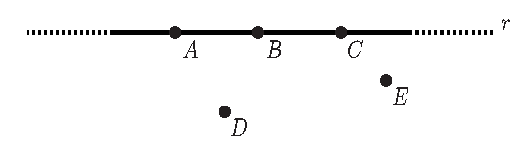
\includegraphics[trim=0cm 0cm 0cm 0cm,clip,scale=0.50]{images/fivepointconic1.pdf}
	\end{minipage}\\
	\begin{minipage}{0.69\textwidth}
	Escludiamo $C$ e consideriamo $A,\ B,\ D,\ E$:
	\begin{itemize}
		\item Sono in posizione generale: siamo a posto.
		\item Tre sono allineati.
	\end{itemize}
	Abbiamo già che $D,E \notin r$, dunque i tre punti allineati possono essere $A,\ D,\ E$ oppure $B,\ D,\ E$. Supponendo siano $A,\ D,\ E$, scartiamo $A$ e otteniamo $B,\ C,\ D,\ E$ in posizione generale.
	\end{minipage}
	%\hspace{-12mm}
	\begin{minipage}{0.30\textwidth}
		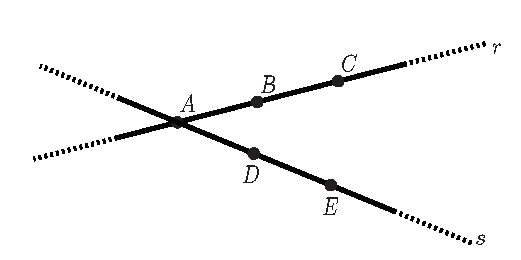
\includegraphics[trim=0cm 0cm 0cm 0cm,clip,scale=0.50]{images/fivepointconic2.pdf}
	\end{minipage}\\
	Possiamo ora applicare la proposizione precedente: sia $\mathcal{F}$ il fascio delle coniche passanti per $A,\ B,\ C,\ D$; poiché $E$ non è un punto base per $\mathcal{F}$ in quanto i punti base sono i cinque punti $A,\ B,\ C,\ D$, esiste ed è \textit{unica} la conica $C$ del fascio che passa per $E$. $C$ è l'unica conica che contiene i cinque punti.
\end{demonstration}
Questa dimostrazione dà anche il metodo per trovare la conica che passa per tali 5 punti.
\begin{tips}
	Per trovare una conica $\mathcal{C}$ che passa per 5 punti dati $A,\ B,\ C,\ D,\ E$ in $\proj[2]{\ }$ potremmo partire dalla conica generale e imporre il passaggio per 5 punti, ma è un calcolo laborioso. Un metodo più rapido è invece il seguente.
		\begin{itemize}
			\item	Scegliere quattro punti in posizione generale $A,\ B,\ C,\ D$.
			\item	Scrivere quattro rette e il fascio $\mathcal{F} $ come nel ‘‘Tips \& Tricks!'' a pag. \pageref{fascio coniche per 4 pt pos gen}.
			\item	Imporre il passaggio per il quinto punto $E$ in modo da trovare la conica $\mathcal{C}$.
		\end{itemize}
	\vspace{-3mm}
\end{tips}
\begin{observe}
	Il passaggio per un punto di una conica generica dà \textit{equazioni lineari omogenee} sui coefficienti della conica; possiamo pensarlo dunque come un \textit{iperpiano} in $\proj[5]{\ }$. È ragionevole aspettarsi che con cinque punti ho cinque iperpiani che, in posizione generale, si intersecano in solo punto.\\
	L'ipotesi sui punti a 4 a 4 non allineati serve a garantire che le condizioni lineari siano \textit{indipendenti}, così da ottenere un punto solo nell'intersezione degli iperpiani.
\end{observe}
\begin{example}~{}\\
		\begin{minipage}{0.69\textwidth}
	Se abbiamo 5 punti di cui 4 allineati su una retta $r$, allora per ogni retta $s$ che passa per $P$ la conica $r\cup s$ contiene i 5 punti, quindi ci sono \textit{infinite coniche} avendo infinite rette $s$.
	\end{minipage}
	%\hspace{-1mm}
	\begin{minipage}{0.3\textwidth}
		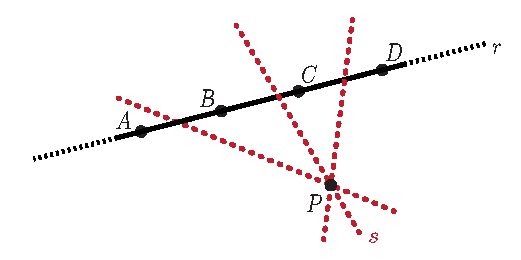
\includegraphics[trim=0cm 0cm 0cm 0cm,clip,scale=0.50]{images/fourpointconic.pdf}
	\end{minipage}
\end{example}
\begin{proposition}[Fascio di coniche per 3 punti non allineati e una retta tangente.]~{}\\~{}\\
	\begin{minipage}{0.72\textwidth}
	Siano 3 punti \textit{non allineati} $A,\ B,\ C\in\proj[2]{\ }$, e sia una retta $r$ che passi per $A$ ma non per $B$ e $C$, ovvero $A\in r$ e $B,\ C\notin r$. La famiglia delle coniche che passano per $A,\ B,\ C$ e sono tangenti a $r$ in $A$ è un fascio $\mathcal{F}$.\\
	I punti base del fascio $\mathcal{F}$ sono solo $A,\ B,\ C$; il fascio \textit{non} contiene rette doppie e ci sono solo due coniche degeneri $\overline{AB}\cup\overline{AC}$ e $r\cup\overline{BC}$.
	\end{minipage}
	\hspace{-2mm}
	\begin{minipage}{0.27\textwidth}
		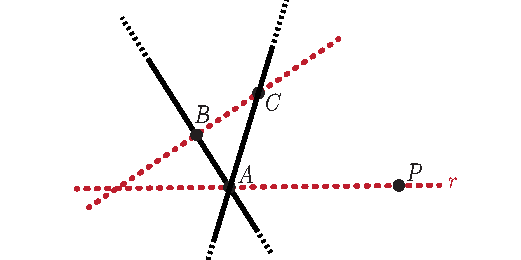
\includegraphics[trim=0cm 0cm 0cm 0cm,clip,scale=0.50]{images/fourpointconic2.pdf}
	\end{minipage}
\end{proposition}
\begin{demonstration}
	Sia $P\in r$ un punto diverso da $A$ e $P\notin\overline{BC}$. $A,\ B,\ C,\ P$ sono in posizione generale, perché a tre a tre non allineati. Scegliamo le coordinate proiettive tali che $A,\ B,\ C$ siano i punti coordinati mentre $P$ il punto unità: $A=(1\colon 0\colon 0),B=(0\colon 1\colon 0),C=(0\colon 0\colon 0\colon1)$.
	Allora la retta $r=\overline{AP}$ ha equazione $x_1-x_2=0$.\\
	Si consideri la conica generale:
	\begin{equation*}
		a_{00}x_0^2+2a_{01}x_0x_1+a_{11}x_1^2+2a_{02}x_0x_2+2a_{12}x_1x_2+a_{22}x_2^2=0
	\end{equation*}
	Sappiamo già che il passaggio per i punti coordinati annulla la diagonale della matrice associata:
	\begin{equation*}
		\begin{array}{ll}
			\text{Per } A \colon & a_{00}=0 \\
			\text{Per } B \colon & a_{11}=0 \\
			\text{Per } C \colon & a_{22}=0 \\
		\end{array}
	\implies F=a_{01}x_0x_1+a_{12}x_1x_2+a_{02}x_0x_2
	\end{equation*}
	Intersechiamo con $r\colon x_1=x_2$ e sostituiamo in $F$:
	\begin{equation*}
		a_{01}x_0x_+a_{12}x_1^2+a_{02}x_0x_1=0\implies x_1((a_{01}+a_{02})x_0+a_{12}x_1)=0
	\end{equation*}
	Notiamo che $x_1=0$ è dovuto al fatto che $A\in r\cap C$. Ne segue che $r$ è tangente alla conica in $A$ se e solo se $A$ ha molteplicità due, quindi se e solo $x_1=0$ è l'unica soluzione. Necessariamente il coefficiente di $x_0$ nell'equazione precedente deve essere nullo, cioè $a_{01}+a_{02}=0\implies a_{02}=-a_{01}$. Sostituendo nell'equazione si ottiene:
		\begin{equation*}
			a_{01}x_0x_1 -a_{01}x_0x_2 + a_{12}x_1x_2=0 \implies a_{01}x_0(x_1-x_2) + a_{12}x_1x_2=0
		\end{equation*}
	Quest'equazione descrive tutte e sole le coniche per $A,\ B,\ C$ e tangenti a $r$ in $A$; in questo modo abbiamo verificato che è un fascio $\mathcal{F}$.\\
	Le coniche che lo generano sono $C_1\colon \underbrace{x_0}_{\overline{BC}} \underbrace{(x_1-x_2)}_{r}$ e $C_2\colon \underbrace{x_1}_{\overline{AC}} \underbrace{x_2}_{\overline{AB}}$. Intersecando $C_1$ e $C_2$ otteniamo i punti base:
		\begin{gather*}
			C_1\cap C_2 = (\overline{BC}\cup r) \cap (\overline{AC}\cup\overline{AB})=(\overline{BC}\cap\overline{AC}) \cup (\overline{BC}\cap\overline{AB}) \cup (r\cap\overline{AC}) \cup (r\cap\overline{AB}) =\{ C,B,A \}
		\end{gather*}
	Scriviamo la matrice per verificare che non ci siano altre coniche degeneri e altri punti base:
		\begin{gather*}
			M=\begin{pmatrix}
				0 & a_{01} & -a_{01}\\
				a_{01} & 0 & a_{12}\\
				-a_{01} & a_{12} & 0
			\end{pmatrix}\\
			D=\det M= -a_{01}(a_{01}a_{12}) -a_{01}(a_{01}a_{12}) = -2a_{01}^2 a_{12}
		\end{gather*}
	Siccome $D$ è un polinomio omogeneo di grado 3 si ha una radice doppia, ma le due radici danno le coniche che generano il fascio e dunque le uniche coniche degeneri sono solo $C_1$ e $C_2$.
	% \footnote{Le due coppie di rette soddisfano le condizioni necessarie: nella prima si intersecano in $A$ e la molteplicità di intersezione è 2, conta 1 per ciascuna retta, pertanto la retta è tangente, dal punto di vista dei punti singolari invece la retta è singolare, e ogni retta per $A$ è tangente; mentre la seconda coppia passa per $A,\ B,\ C$ e contiene $r$, dunque siccome quando è contenuta è tangente si ha molteplicità infinita.}
\end{demonstration}

\begin{observe}
	Un fascio di questo tipo è il primo esempio a pag. \pageref{esempi lez 35}.\\
	\begin{minipage}{0.72\textwidth}
	Consideriamo $C_1\colon x_0x_1=0$ e $C_2\colon (x_0-x_1)x_2=0$. Allora, la retta $x_0-x_1=0$ passa per il punto di intersezione delle prime due rette $x_0=0$ e $X_1=0$, quindi siamo nella situazione precedente: $A$ è il punto di intersezione, mentre $B$ e $C$ sono i punti di intersezione di $x_2=0$ con $x_0=0$ e $x_1=0$. Dunque $C_2$ diventa $r\cup \overline{BC}$, mentre $C_1$ è $\overline{AB}\cup \overline{AC}$.
	\end{minipage}
	\hspace{-5mm}
	\begin{minipage}{0.27\textwidth}
		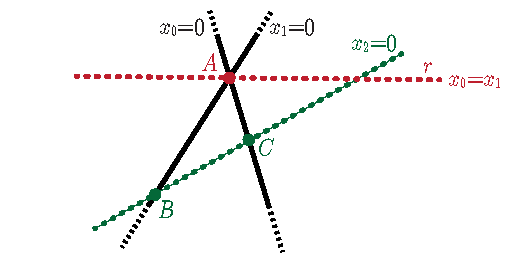
\includegraphics[trim=0cm 0cm 0cm 0cm,clip,scale=0.50]{images/fourpointconic3.pdf}
	\end{minipage}\\
Abbiamo già verificato che i punti base sono solo $A,\ B,\ C$ e che $C_1$ e $C_2$ sono le uniche coniche degeneri di $\mathcal{F}$ ed ora osserviamo che la retta $r$ è tangente a tutte le coniche del fascio.
\end{observe}
%DISEGNO
\subsection{Impratichiamoci! Fasci di coniche proiettive}
\begin{exercise} \textsc{F.F.P., 2.1.}\\
	Nel piano proiettivo reale $\proj[2]{\realset}$ consideriamo i punti:
	\begin{equation*}
		A=(0\colon 1 \colon 2),\ B=(0\colon 0\colon 1),\ C=(2\colon1\colon2),\ D=(3\colon0\colon1)
	\end{equation*}
	Determinare, se esiste, l'equazione di una conica passante per $A,\ B,\ C,\ D$ e tangente in $C$ alla retta $r$ di equazione $x_0-x_2=0$ che passa per $C$.
\end{exercise}
\begin{solution}
	Controlliamo che i 4 punti siano in posizione generale verificando,  con i determinanti, che siano a 3 a 3 non allineati:
		\begin{equation*}
			\begin{array}{ll}
				\begin{vmatrix}
					0 & 0 & 2\\
					1 & 0 & 1\\
					2 & 1 & 2
				\end{vmatrix} \neq 0 \implies A,\ B,\ C \text{ non allineati} &
				\quad\begin{vmatrix}
					0 & 0 & 3\\
					1 & 0 & 0\\
					2 & 1 & 1
				\end{vmatrix} \neq 0 \implies A,\ B,\ D \text{ non allineati} \\
			\begin{vmatrix}
				0 & 2 & 3\\
				0 & 1 & 0\\
				1 & 2 & 1
			\end{vmatrix} \neq 0 \implies B,\ C,\ D \text{ non allineati} &
			\quad \begin{vmatrix}
				0 & 2 & 3\\
				1 & 1 & 0\\
				2 & 2 & 1
			\end{vmatrix} \neq 0 \implies A,\ C,\ D \text{ non allineati}
			\end{array}
		\end{equation*}
	Dunque c'è un fascio $\mathcal{F}$ di coniche per $A,\ B,\ C,\ D$. Scriviamo l'equazione delle quattro rette con il determinante formale delle coordinate:
		\begin{gather*}
			\begin{array}{lll}
			\text{Retta } \overline{AB} \colon & \begin{vmatrix}
					x_0 & x_1 & x_2 \\
					0 & 1 & 2 \\
					0 & 0 & 1
				\end{vmatrix} & = x_0=0\\
			\text{Retta } \overline{CD} \colon & \begin{vmatrix}
				x_0 & x_1 & x_2 \\
				2 & 1 & 2 \\
				3 & 0 & 1
			\end{vmatrix} & = x_0- x_1 (-4) + x_2(-3)=x_0 +4x_1-3x_2=0\\
			&& \implies C_1\colon x_0(x_0+4x_1-3x_2)\\
			\text{Retta } \overline{BD} \colon & \begin{vmatrix}
					x_0 & x_1 & x_2 \\
					0 & 0 & 1 \\
					3 & 0 & 1
				\end{vmatrix} & = x_1=0\\
				\text{Retta } \overline{AC} \colon & \begin{vmatrix}
					x_0 & x_1 & x_2 \\
					0 & 1 & 2 \\
					2 & 1 & 2
				\end{vmatrix} & = -x_1(-4) +x_2(-2)= 4x_1 -2x_2=0 \implies 2x_1-x_2=0\\
			&& \implies C_2 \colon x_1(2x_1-x_2) \\
			\end{array}\\
			\text{fascio } \mathcal{F}\colon \lambda x_0(x_0+4x_1-3x_2) +\mu x_1(2x_1-x_2)=0
		\end{gather*}
	Queste sono tutte e sole le coniche che passano per $A,\ D$. Vogliamo la conica del fascio che è tangente alla retta $r\colon x_0-x_2=0$ in $C$. Intersechiamo la conica $C_{\lambda,\mu}$ con la retta $r$ sostituendo $x_2=x_0$ nell'equazione:
		\begin{equation*}
			\begin{array}{lll}
				\lambda x_0(x_0+4x_1-3x_0)+\mu x_1(2x_1-x_0)=0 & \implies & \lambda x_0(4x_1-2x_0)+ \mu x_1(2x_1-x_0)=0\\
				\implies 2\lambda x_0(2x_1-x_0)+ \mu x_1(2x_1-x_0)=0 & \implies & (2x_1-x_0)(2\lambda x_0 +\mu x_1)=0
			\end{array}
		\end{equation*}
	Sostituendo $x_2=x_0$ stiamo parametrizzando la retta $r$ come $(x_0\colon x_1\colon x_0)$. Il passaggio per $C=(2\colon1\colon2)$ corrisponde al primo fattore $x_0=2x_1$. Pertanto, la retta $r$ è tangente alla conica nel punto $C$ se e solo se anche l'altra soluzione corrisponde al punto $C$, cioè se e solo se $2\lambda x_0 +\mu x_1$ e $-x_0+2x_1$ sono proporzionali:
	\begin{equation*}
		\det \begin{pmatrix}
			2\lambda & \mu \\
			-1 & 2
		\end{pmatrix} =0 \iff 4\lambda +\mu=0 \implies \mu=-4\lambda
	\end{equation*}
	Ad esempio, per $\lambda=1$ e $\mu=-4$ si ha $2\lambda x_0+\mu x_1=2x_0-4x_1$. L'equazione della conica sarà $\mathcal{C} \colon x_0(x_0+4x_1-3x_2) -4x_1(2x_1-x_2)=0 \implies \mathcal{C}\colon x_0^2 +4x_0x_1 -3x_0x_2 -8x_1^2 +4x_1x_2=0$, dunque esiste ed è unica la conica cercata.\\
	Controlliamo se la conica fa quello che deve fare. Passa per i punti dati? Sì, infatti:
	\begin{equation*}
		\begin{array}{ll}
			F(A)=F(0,1,2)=-8+8=0 & F(B)=F(0,0,1)=0 \\
			F(C)=F(2,1,2)= 4+8-12-8+8 =0 & F(D)=F(3,0,1)=9-9=0
		\end{array}
	\end{equation*}
	È tangente a $r$ in $C$? Scriviamo direttamente la tangente alla conica nel punto $C=(2\colon1\colon2)$ con le derivate parziali:
		\begin{gather*}
			\begin{array}{lll}
				\frac{\partial{F}}{\partial{x_0}} = 2x_0+4x_1-3x_2 & \frac{\partial{F}}{\partial{x_1}} = 4x_0-16 x_1 +4x_2 & \frac{\partial{F}}{\partial{x_2}} = -3x_0 +ax_1\\
				\frac{\partial{F}}{\partial{x_0}} (2,1,2) =4+4-6=2 & \frac{\partial{F}}{\partial{x_1}} (2,1,2) =8-16+6=0 & \frac{\partial{F}}{\partial{x_2}} (2,1,2) = -6+4=2\\
			\end{array}\\
			\implies 2x_0-2x_2=0 \implies x_0-x_2=0
		\end{gather*}
	Otteniamo proprio la retta $r$.
\end{solution}
